\documentclass[UTF8,a4paper,12pt]{ctexbook} 

\usepackage{graphicx}%学习插入图
\usepackage{verbatim}%学习注释多行
\usepackage{booktabs}%表格
\usepackage{geometry}%图片
\usepackage{amsmath}
\usepackage{amssymb}
\usepackage{listings}%代码
\usepackage{xcolor}  %颜色
\usepackage{enumitem}%列表格式
\setenumerate[1]{itemsep=0pt,partopsep=0pt,parsep=\parskip,topsep=5pt}
\setitemize[1]{itemsep=0pt,partopsep=0pt,parsep=\parskip,topsep=5pt}
\setdescription{itemsep=0pt,partopsep=0pt,parsep=\parskip,topsep=5pt}
\usepackage{tcolorbox}
\usepackage{algorithm}  %format of the algorithm
\usepackage{algorithmic}%format of the algorithm
\usepackage{multirow}   %multirow for format of table
\usepackage{tabularx} 	%表格排版格式控制
\usepackage{array}	%表格排版格式控制
\usepackage{hyperref} %超链接 \url{URL}
\usepackage{tikz}
\usepackage{dirtree}

\CTEXsetup[format+={\flushleft}]{section}

%%%% 设置图片目录
\graphicspath{{figure/}}

%%%% 段落首行缩进两个字 %%%%
\makeatletter
\let\@afterindentfalse\@afterindenttrue
\@afterindenttrue
\makeatother
\setlength{\parindent}{2em}  %中文缩进两个汉字位

%%%% 下面的命令重定义页面边距,使其符合中文刊物习惯 %%%%
\addtolength{\topmargin}{-54pt}
\setlength{\oddsidemargin}{0.63cm}  % 3.17cm - 1 inch
\setlength{\evensidemargin}{\oddsidemargin}
\setlength{\textwidth}{14.66cm}
\setlength{\textheight}{24.00cm}    % 24.62

%%%% 下面的命令设置行间距与段落间距 %%%%
\linespread{1.0}
\setlength{\parskip}{0.5\baselineskip}
\geometry{left=1.6cm,right=1.8cm,top=2cm,bottom=1.7cm} %设置文章宽度
\pagestyle{plain} 		  %设置页面布局

%代码效果定义
\definecolor{mygreen}{rgb}{0,0.6,0}
\definecolor{mygray}{rgb}{0.5,0.5,0.5}
\definecolor{mymauve}{rgb}{0.58,0,0.82}
\lstset{ %
	backgroundcolor=\color{white},   % choose the background color
	basicstyle=\footnotesize\ttfamily,      % size of fonts used for the code
	%stringstyle=\color{codepurple},
	%basicstyle=\footnotesize,
	%breakatwhitespace=false,         
	%breaklines=true,                 
	%captionpos=b,                    
	%keepspaces=true,                 
	%numbers=left,                    
	%numbersep=5pt,                  
	%showspaces=false,                
	%showstringspaces=false,
	%showtabs=false,        
	columns=fixed,
	breaklines=true,                 % automatic line breaking only at whitespace
	captionpos=b,                    % sets the caption-position to bottom
	tabsize=4,
	commentstyle=\color{mygreen},    % comment style
	escapeinside={\%*}{*)},          % if you want to add LaTeX within your code
	keywordstyle=\color{blue},       % keyword style
	stringstyle=\color{mymauve}\ttfamily,     % string literal style
	frame=L,
	xleftmargin = .04\textwidth,
	rulesepcolor=\color{red!20!green!20!blue!20},
	% identifierstyle=\color{red},
	language=c++,
}
 \author{\kaishu 郑华}
 \title{\heiti OpenGL 学习笔记}

\begin{document}          %正文排版开始
 	\maketitle
 
	\newpage
	\tableofcontents
	
\newpage
\chapter{安装配置}
    \section{各种库文件}网盘环境
    \textbf{有时一个warnning可能就会导致全局皆输。}
    
    比如这次环境的调试程序,一个warnning4005  就是隐式转类型警告,结果就是跑不出来。最后发现是OpenGL为了兼容各系统,估计是把每个类型的字节固定了,而且还是32位,而我的是64位,导致了程序的不可运行
    
    \section{常见错误}
	    \subsection{0x70000000C}见图\ref{Glut Error},图\ref{Glut_fix}.
	    
		    解决:1- 使用glut.h , 2- 给链接输入添加\verb|glut32.lib Opengl32.lib Glu32.lib glew32.lib comctl32.lib|
		    \begin{figure}[h]
		    	\begin{center}
					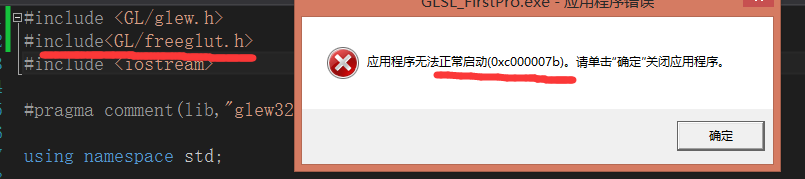
\includegraphics[scale = 0.5]{glutDoesNotMatchError.png}%就在前面括号中写图片名
		    		\caption{Error}
		    		\label{Glut Error}
		    	\end{center}
		    \end{figure}
		    \begin{figure}[h]
		    	\centering
		    	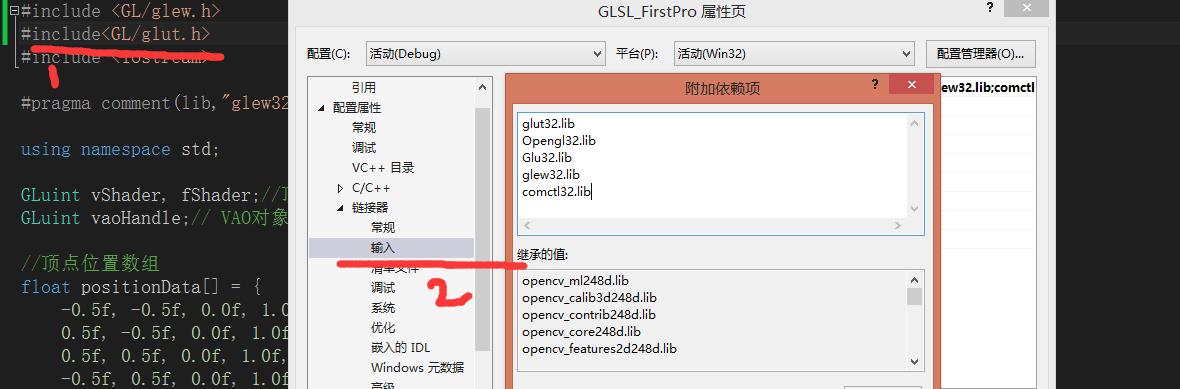
\includegraphics[scale = 0.4]{glutMatch.png}
		    	\caption{解决方法}
		    	\label{Glut_fix}
		    \end{figure}
		    
		\subsection{使用glut 与 glew 不兼容报0x0000005}
			
			改用glfw 调用窗口即可。
		
			\begin{lstlisting}
#include <iostream>
#include <Windows.h>  
#include <GL/glew.h>    
#include <GLFW/glfw3.h>   

GLuint WIDTH = 720, HEIGHT = 720;
unsigned int VBO, VAO, EBO, UBO, FBO;

const char *vertexShaderSource = "#version 330 core\n"
"layout (location = 0) in vec3 aPos;\n"
"void main()\n"
"{\n"
"   gl_Position = vec4(aPos.x, aPos.y, aPos.z, 1.0);\n"
"}\0";
const char *fragmentShaderSource = "#version 330 core\n"
"out vec4 FragColor;\n"
"void main()\n"
"{\n"
"   FragColor = vec4(1.0f, 0.5f, 0.2f, 1.0f);\n"
"}\n\0";


float vertexData[] = {
	-0.5f, 0, 0,
	0.5f,  0, 0,
	0,  0.5f, 0,
};


void initVAOetc()
{
	glGenVertexArrays(1, &VAO);	// 顶点缓冲+顶点读取方式 统一索引
	glGenBuffers(1, &VBO);	// 顶点缓冲
	glBindVertexArray(VAO);
	glBindBuffer(GL_ARRAY_BUFFER, VBO);
	glBufferData(GL_ARRAY_BUFFER, sizeof(vertexData), vertexData, GL_STATIC_DRAW);	// 顶点数据
	glVertexAttribPointer(0, 3, GL_FLOAT, GL_FALSE, 3 * sizeof(float), (void*)0);	// 顶点读取方式
	glEnableVertexAttribArray(0);
	glBindBuffer(GL_ARRAY_BUFFER, 0);
	glBindVertexArray(0);
}


int main()
{
	glfwInit();

	GLFWwindow* window = glfwCreateWindow(WIDTH, HEIGHT, "OpenGL", nullptr, nullptr);
	if (window == nullptr)
	{
		std::cout << "Failed to create GLFW window" << std::endl;
		glfwTerminate();
		return -1;
	}

	glfwMakeContextCurrent(window);

	if (glewInit() != GLEW_OK)
	{
		std::cout << "Failed to initialize GLEW" << std::endl;
		return -1;
	}

	glViewport(0, 0, WIDTH, HEIGHT);
	initVAOetc();

	// 渲染loop   
	while (!glfwWindowShouldClose(window))
	{
		glfwPollEvents();//通知处理窗口事件,注释掉的话,窗口可能会卡住
		glClearColor(0.0f, 0.0f, 0.0f, 1.0f);//指定一种颜色清屏
		glClear(GL_COLOR_BUFFER_BIT);//清屏
		
		glBindVertexArray(VAO);
		glDrawArrays(GL_TRIANGLES, 0, 3);
		glBindVertexArray(0);

		glfwSwapBuffers(window);//是opengl绘制的图形显示在窗口上
	}


	glfwTerminate();//窗口结束
	return 0;
}				
			\end{lstlisting}  
		    
    \section{参考文献} 
    \url{http://johnhany.net/2015/03/environment-for-opengl-4-with-vs2012/}    
    
    win10+nugPackage:\url{https://www.cnblogs.com/flylinmu/p/7823019.html}
    


\newpage
\chapter{图形学基础}
	完全指南:\url{https://www.jianshu.com/p/6bda18e953f6}
	
	API:\url{https://www.khronos.org/opengl/wiki/Category:Core_API_Reference}
	
	\section{OpenGL 框架结构}
		\begin{figure}[H]
			\centering
			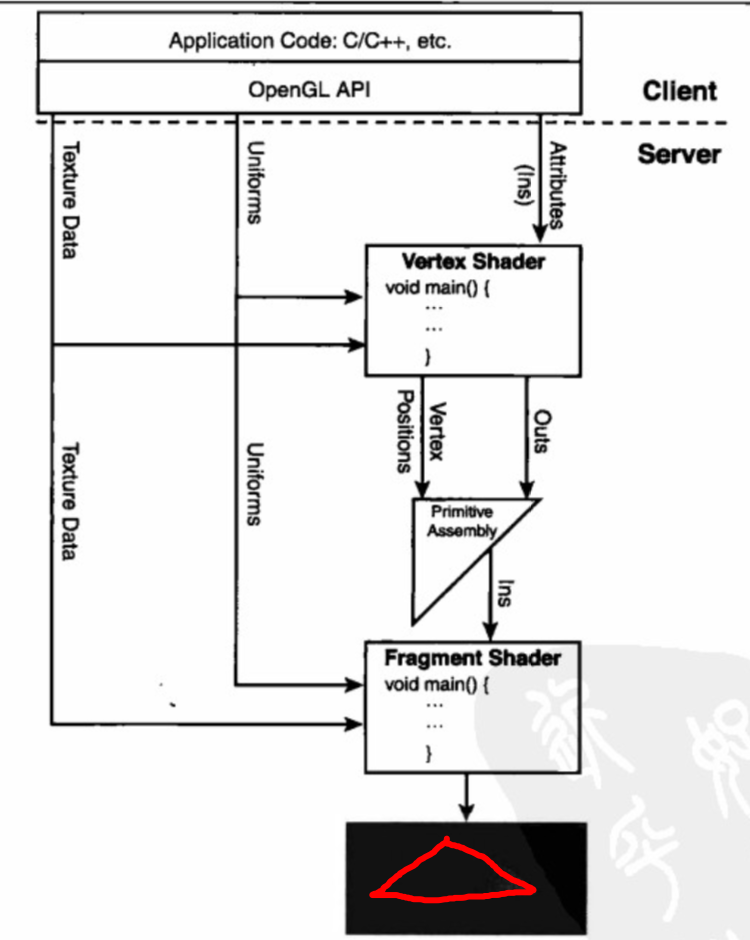
\includegraphics[width=.91\linewidth]{openGlArch}
			\caption{基本渲染框架}
		\end{figure}
			
				
	\section{绘制三角形}
	
		\subsection{流程}
			任何事物都在3D空间中,而屏幕和窗口却是2D像素数组,这导致OpenGL的大部分工作都是关于把3D坐标转变为适应你屏幕的2D像素。
			
			3D坐标转为2D坐标的处理过程是由OpenGL的图形\textbf{渲染管线}(Graphics Pipeline,指的是\textbf{一堆原始图形数据}途经一个输送管道,期间\textbf{经过各种变化处理}最终\textit{出现在屏幕的过程})管理的。图形渲染管线可以被划分为两个主要部分:
				\begin{itemize}[itemindent = 1em]
					\item 第一部分把你的3D坐标转换为2D坐标
					\item 第二部分是把2D坐标转变为实际的有颜色的像素
				\end{itemize}
			
			\begin{figure}[H]
				\centering
				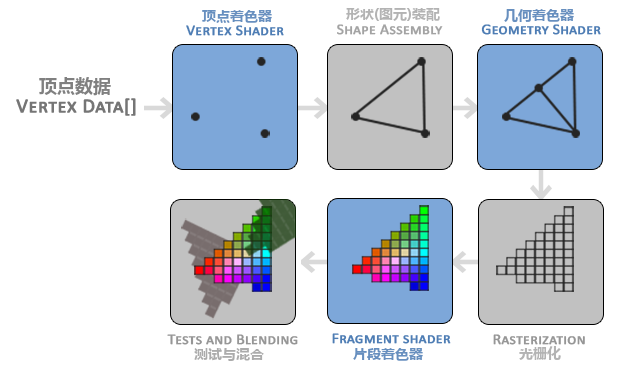
\includegraphics[width=.93\linewidth]{PipelineBase}
				\caption{Graphics Pipeline}
			\end{figure}

			
			因而对应的,在第一部分需要输入\textbf{顶点数据}。而第二部分则需要\textbf{第一部分转换坐标后的点}+\textbf{颜色处理程序}。
			
		
		\subsection{顶点数据-输入-GPU显存}
			
			\paragraph{概述}
				首先,我们以数组的形式传递3个3D坐标作为图形渲染管线的输入,用来表示一个三角形,这个数组叫做顶点数据(Vertex Data);顶点数据是一系列顶点的集合。
				\textbf{顶点数据buffer}。
				
				一个顶点(Vertex)是一个3D坐标的数据的集合。顶点数据是用顶点属性(Vertex Attribute)表示的,它可以包含任何我们想用的数据。
				
				任何一个绘制指令的调用都需要将\textbf{图元信息}传递给OpenGL。这是其中的几个:\verb|GL_POINTS|、\verb|GL_TRIANGLES|、\verb|GL_LINE_STRIP|。
				
			\paragraph{API 示例}
			
				\subparagraph{准备顶点数据}
					首先需要定义顶点数据,\textit{OpenGL仅当3D坐标在3个轴(x、y和z)上都为-1.0到1.0的范围内时才处理它}。所有在所谓的\textbf{标准化设备坐标}(Normalized Device Coordinates)范围内(\verb|-1~1|)的坐标才会最终呈现在屏幕上(在这个范围以外的坐标都不会显示)。
					
					\begin{lstlisting}
float vertices[] = {
    -0.5f, -0.5f, 0.0f,
     0.5f, -0.5f, 0.0f,
     0.0f,  0.5f, 0.0f
};				
					\end{lstlisting}
					
					以后,需要把它\textit{作为输入}\textbf{发送给}图形渲染管线的第一个处理阶段:顶点着色器,它会在\textbf{GPU}上创建内存用于储存我们的顶点数据。
					
					我们通过\textbf{顶点缓冲对象(Vertex Buffer Objects, VBO)}管理这个内存,它会在GPU内存(通常被称为显存)中储存大量顶点。使用这些缓冲对象的好处是我们可以一次性的发送一大批数据到显卡上,而不是每个顶点发送一次。
					
					OpenGL中的对象,都有一个独一无二的ID。所以对于顶点缓冲对象,同样具有一个对象ID,可以使用glGenBuffers函数生成一个VBO \textit{空}对象(\textit{未初始化、未绑定数据}),并获取其对象ID:
					
					\begin{lstlisting}
unsigned int VBO;
glGenBuffers(1, &VBO);				
					\end{lstlisting}
					
					OpenGL中有很多缓存对象,虽然它给了我们一个ID,但不知道这个ID是用来表示什么缓存对象的。所以需要手动明确告诉它,初始化它的类型字段(用途),这是一个顶点缓存对象。顶点缓冲对象的缓冲类型是\verb|GL_ARRAY_BUFFER|。OpenGL\textit{允许同时绑定多个缓冲},\textbf{只要}它们是不同的缓冲类型。使用\textbf{glBindBuffer()函数}把新创建的\textit{缓冲对象}绑定到\verb|GL_ARRAY_BUFFER|目标上.
					
					\begin{lstlisting}
glBindBuffer(GL_ARRAY_BUFFER, VBO);
					\end{lstlisting}
					
					\underline{从这一刻起},我们\textbf{使用的任何}(在\verb|GL_ARRAY_BUFFER|\textit{目标上的})\textbf{缓冲调用}\underline{都会}\textit{用来配置当前绑定的缓冲}(VBO)。然后我们可以调用\textbf{glBufferData()函数},它会把之前定义的顶点数据复制到缓冲的显存中。
					
					\begin{lstlisting}
glBufferData(GL_ARRAY_BUFFER, sizeof(vertices), vertices, GL_STATIC_DRAW);					
					\end{lstlisting}
								
							
				\subparagraph{设置顶点数据解释格式}
					\textit{顶点着色器}\underline{允许}我们指定\textit{任何形式}的\textit{顶点属性}为\textbf{输入}。这使其具有很强的灵活性的同时,它还的确意味着我们必须手动指定输入数据的哪一个部分对应顶点着色器的哪一个顶点属性。所以,我们\textbf{必须在渲染前(绘画前)}\underline{确定或设置好}OpenGL解释顶点数据的\textbf{模版}。	
						
					这个工作由\textbf{glVertexAttribPointer()函数}完成。	
					
					\begin{lstlisting}
glVertexAttribPointer(0, 3, GL_FLOAT, GL_FALSE, 3 * sizeof(float), (void*)0);
					\end{lstlisting}
					
					\begin{itemize}
						\item 第一个参数指定顶点属性位置,与顶点着色器中layout(location=0)对应,注意,这里的顶点属性是一个数组,存储多种属性,如位置0存放位置、位置1存放颜色、位置2存放纹理坐标等。
						\item 第二个参数指定顶点属性大小。顶点属性是一个vec3,它由3个值组成,所以大小是3。
						\item 第三个参数指定数据类型。
						\item 第四个参数定义是否希望数据被标准化。
						\item 第五个参数是步长(Stride),指定在连续的顶点属性之间的间隔,\textit{单位字节}。
						\item 第六个参数表示我们的位置数据在缓冲区起始位置的偏移量。决定怎么取不同属性的核心参数,与第2个参数呼应。
					\end{itemize}
					
					顶点属性\verb|glVertexAttribPointer|默认是关闭的,使用时要以顶点属性位置值为参数调用\verb|glEnableVertexAttribArray()|开启。
					
					
					使用示例:
					\begin{lstlisting}
float vertices[] = {
    // positions          // colors           // texture coords
     0.5f,  0.5f, 0.0f,   1.0f, 0.0f, 0.0f,   1.0f, 1.0f, // top right
     0.5f, -0.5f, 0.0f,   0.0f, 1.0f, 0.0f,   1.0f, 0.0f, // bottom right
    -0.5f, -0.5f, 0.0f,   0.0f, 0.0f, 1.0f,   0.0f, 0.0f, // bottom left
    -0.5f,  0.5f, 0.0f,   1.0f, 1.0f, 0.0f,   0.0f, 1.0f  // top left 
};
 
// position attribute
glVertexAttribPointer(0, 3, GL_FLOAT, GL_FALSE, 8 * sizeof(float), (void*)0);
glEnableVertexAttribArray(0);
// color attribute
glVertexAttribPointer(1, 3, GL_FLOAT, GL_FALSE, 8 * sizeof(float), (void*)(3 * sizeof(float)));
glEnableVertexAttribArray(1);
// texture coord attribute
glVertexAttribPointer(2, 2, GL_FLOAT, GL_FALSE, 8 * sizeof(float), (void*)(6 * sizeof(float)));
glEnableVertexAttribArray(2);   	
					\end{lstlisting}
					
					
					对应的顶点着色器如下:
					\begin{lstlisting}
#version 330 core
layout (location = 0) in vec3 aPos;
layout (location = 1) in vec3 aColor;
layout (location = 2) in vec2 aTexCoord;

out vec3 ourColor;
out vec2 TexCoord;

void main()
{
    gl_Position = vec4(aPos, 1.0);
    ourColor = aColor;
    TexCoord = aTexCoord;
}					
					\end{lstlisting}
					
					对应的内存布局如下(\textit{少了纹理的属性2}):
					
					\begin{figure}[H]
						\centering
						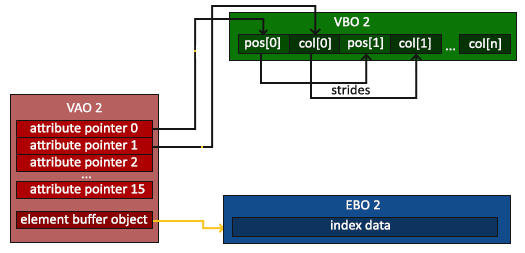
\includegraphics[width=.9\linewidth]{vertexAttribute}
					\end{figure}
					
					
					
					
					
					
					
				\subparagraph{VAO-属性保存}	
					VBO保存了\underline{一个模型}的\textit{顶点属性信息},每次绘制模型之前需要绑定顶点的所有信息,当数据量很大时,重复这样的动作变得非常麻烦。
					
					VAO可以把这些所有的配置都存储在一个对象中,\textbf{每次绘制模型时,只需要绑定这个VAO对象就可以了}。
					
					OpenGL的核心模式\textbf{要求我们使用VAO},所以它知道该如何处理我们的顶点输入。\textbf{如果我们绑定VAO失败,OpenGL会拒绝绘制任何东西}。
					
					\begin{lstlisting}
glGenVertexArrays(1, &VAO);			
glBindVertexArray(VAO);		
					\end{lstlisting}
					
					VAO是一个保存了 顶点数据的格式 以及 顶点数据所需的VBO对象的引用,简言之,一个顶点数组对象会储存以下这些内容:
					\begin{enumerate}
						\item \verb|glEnableVertexAttribArray|和\verb|glDisableVertexAttribArray|的调用
						\item 通过\verb|glVertexAttribPointer()|设置的 \textbf{顶点属性格式配置}。
						\item 与顶点属性 关联的 \textbf{顶点缓冲对象(VBO)}
					\end{enumerate}
					
					
					\begin{figure}[H]
						\centering
						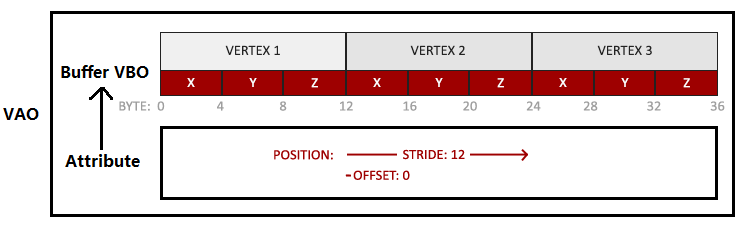
\includegraphics[width=\linewidth]{VBO_Attr}
						\caption{VAO 数据模型示例}
					\end{figure}
					
				\subparagraph{VAO-设置与初始化}		
					具体就是绑定VBO与顶点属性,如下:
					\begin{lstlisting}
void initVAOetc()
{
	glGenVertexArrays(1, &VAO);	// 顶点缓冲+顶点读取方式 统一索引
	glGenBuffers(1, &VBO);	// 顶点缓冲
	glBindVertexArray(VAO);
	glBindBuffer(GL_ARRAY_BUFFER, VBO);
	glBufferData(GL_ARRAY_BUFFER, sizeof(vertexData), vertexData, GL_STATIC_DRAW);	// 顶点数据
	glVertexAttribPointer(0, 3, GL_FLOAT, GL_FALSE, 3 * sizeof(float), (void*)0);	// 顶点读取方式
	glEnableVertexAttribArray(0);
	glBindBuffer(GL_ARRAY_BUFFER, 0);
	glBindVertexArray(0);
}					
					\end{lstlisting}
							
		\subsection{GPU-顶点处理}
			\paragraph{概述}		
				图形渲染管线的第一个部分是\textbf{顶点着色器(Vertex Shader)},它把一个单独的\textbf{顶点作为输入}。顶点着色器主要的目的是\textbf{把3D坐标转为另一种3D坐标}(后面会解释),\textit{同时}顶点着色器允许我们\textbf{对顶点属性进行一些基本处理}。
			
			\paragraph{API 示例}
				第一件事是用着色器语言GLSL(OpenGL Shading Language)\textbf{编写顶点着色器},然后\textbf{编译这个着色器},最后\textbf{在程序中使用}它。
				
				\subparagraph{编写顶点着色器}\verb|->|
				
					\begin{lstlisting}
#version 330 core
layout (location = 0) in vec3 aPos;

void main()
{
    gl_Position = vec4(aPos.x, aPos.y, aPos.z, 1.0);
}				
					\end{lstlisting}
					
					使用\textbf{in关键字},在顶点着色器中\textit{声明所有的输入顶点属性}(\textit{Input Vertex Attribute})。现在我们只关心位置(Position)数据,所以只需要一个顶点属性。GLSL有一个\textbf{向量数据类型},它包含\textit{1到4个float分量},包含的数量可以\textit{从它的后缀数字看出来}。由于每个顶点都有一个3D坐标,就创建一个vec3输入变量aPos。同样也通过layout (location = 0)设定了输入变量的位置值(Location)
					
					为了设置顶点着色器的\textbf{输出},必须\textbf{把位置数据赋值给预定义的gl\_Position变量},它在幕后是vec4类型的。\textbf{在main函数的最后,将}\verb|gl_Position|\textbf{设置的值会成为该顶点着色器的\underline{输出}}。由于我们的输入是一个3分量的向量,我们必须把它转换为4分量的。我们可以把vec3的数据作为vec4构造器的参数,同时把w分量设置为1.0f
				
				
				\subparagraph{编译着色器}\verb|->|
				
					\begin{lstlisting}
unsigned int vertexShader;
vertexShader = glCreateShader(GL_VERTEX_SHADER);
glShaderSource(vertexShader, 1, &vertexShaderSource, NULL);
glCompileShader(vertexShader);	

int  success;
char infoLog[512];
glGetShaderiv(vertexShader, GL_COMPILE_STATUS, &success);	
if(!success)
{
    glGetShaderInfoLog(vertexShader, 512, NULL, infoLog);
    std::cout << "ERROR::SHADER::VERTEX::COMPILATION_FAILED\n" << infoLog << std::endl;
}				
					\end{lstlisting}
				
				
				
		\subsection{GPU-图元装配}
			\paragraph{概述}		
				\textbf{图元装配(Primitive Assembly)阶段}\textit{将顶点着色器输出的所有顶点作为输入}(如果是\verb|GL_POINTS|,那么就是一个顶点),\textbf{将所有的点装配成指定图元的形状};本节例子中是一个三角形。
			
				图元装配阶段的输出会传递给\textbf{几何着色器(Geometry Shader)}。几何着色器把图元形式的\textbf{一系列顶点的集合}作为输入,它可以通过\textit{产生新顶点构造出新的(或是其它的)图元来生成其他形状}。
			
			\paragraph{API 示例}
				这个一般在最后绘画的时候将该参数传递进去。
				
				\begin{lstlisting}
glDrawArrays(GL_TRIANGLES, 0, 3);				
				\end{lstlisting}
				
		
		\subsection{GPU-将图元像素化}
			\paragraph{概述}		
				几何着色器的输出会被传入\textbf{光栅化阶段(Rasterization Stage)},这里它会把图元映射为最终屏幕上相应的\textbf{像素},生成供\textbf{片段着色器(Fragment Shader)}使用的片段(Fragment)。在片段着色器运行\textbf{之前}会执行\textbf{裁切(Clipping)}。裁切会\textit{丢弃超出你的视图以外的所有像素},用来提升执行效率。
				
				\verb|Notice-->|\textbf{一个片段}是OpenGL\textbf{渲染一个像素}所需的所有数据。
			
			
		\subsection{GPU-顶点颜色处理}
			\paragraph{概述}		
				片段着色器的主要目的是计算一个像素的最终颜色,这也是所有OpenGL高级效果产生的地方。通常,片段着色器包含3D场景的数据(比如光照、阴影、光的颜色等等),这些数据可以被用来计算最终像素的颜色。
				
				在所有对应\textbf{颜色值确定以后},最终的对象将会被传到最后一个阶段,叫做\textbf{Alpha测试}和\textbf{混合(Blending)阶段}。这个阶段\textbf{检测}\underline{片段}的对应的\textbf{深度}(和\textbf{模板}(Stencil))值,用它们来\textit{判断这个像素是其它物体的前面还是后面,决定是否应该丢弃}。这个阶段\textbf{也会检查alpha值}(alpha值定义了一个物体的透明度)并对物体进行混合(Blend)。所以,即使在片段着色器中计算出来了一个像素输出的颜色,在渲染多个三角形的时候最后的像素颜色也可能完全不同。
				
			\paragraph{API 示例}
				片段着色器(Fragment Shader)是第二个也是最后一个创建的用于渲染三角形的着色器。片段着色器所做的是计算像素最后的颜色输出。为了让事情更简单,示例片段着色器将会一直输出橘黄色。
				
				在计算机图形中\textbf{颜色}被表示为有\textbf{4个元素的数组}:\textit{红色、绿色、蓝色和alpha(透明度)分量},通常缩写为\textbf{RGBA}。当在OpenGL或GLSL中定义一个颜色的时候,我们把颜色每个分量的强度设置在0.0到1.0之间。比如说我们设置红为1.0f,绿为1.0f,我们会得到两个颜色的混合色,即黄色。
				
				\subparagraph{编写片元着色器}\verb|->|
					\begin{lstlisting}
#version 330 core
out vec4 FragColor;

void main()
{
    FragColor = vec4(1.0f, 0.5f, 0.2f, 1.0f);
} 					
					\end{lstlisting}
				
					\underline{片段着色器}\textbf{只需要一个输出变量},这个变量是一个\textit{4分量向量},\textbf{它表示的是最终的输出颜色},我们应该自己将其计算出来。我们可以用\verb| out关键字 |声明输出变量,这里命名为FragColor。下面,将一个alpha值为1.0(1.0代表完全不透明)的\textit{橘黄色的vec4}\underline{赋值给}\textbf{颜色输出}。					
					
					
				\subparagraph{编译片元着色器}
					编译片段着色器的过程与顶点着色器类似,只不过我们使用\verb|GL_FRAGMENT_SHADER|常量作为\textbf{着色器类型}.
					
					\begin{lstlisting}
unsigned int fragmentShader;
fragmentShader = glCreateShader(GL_FRAGMENT_SHADER);
glShaderSource(fragmentShader, 1, &fragmentShaderSource, NULL);
glCompileShader(fragmentShader);					
					\end{lstlisting}
				
				
				\subparagraph{程序使用shader代码}
					\textit{着色器程序对象(Shader Program Object)}\textit{是多个着色器合并之后并最终链接完成的版本}。\textbf{如果要使用刚才编译的着色器我们必须把它们链接(Link)为一个着色器程序对象,然后在渲染对象的时候激活这个着色器程序}。已激活着色器程序的着色器将在我们发送渲染调用的时候被使用,可以调用\verb|glUseProgram()函数|,用刚创建的程序对象作为它的参数,以激活这个程序对象.
					
					在\verb|glUseProgram()函数|调用之后,每个着色器调用和渲染调用都会使用这个程序对象(也就是之前写的着色器)了。
					
					\begin{lstlisting}
unsigned int shaderProgram;
shaderProgram = glCreateProgram();
glAttachShader(shaderProgram, vertexShader);
glAttachShader(shaderProgram, fragmentShader);
glLinkProgram(shaderProgram);	

glGetProgramiv(shaderProgram, GL_LINK_STATUS, &success);
if(!success) {
    glGetProgramInfoLog(shaderProgram, 512, NULL, infoLog);
    ...
}			

glUseProgram(shaderProgram);	
glDeleteShader(vertexShader);
glDeleteShader(fragmentShader);
					\end{lstlisting}
				
				
				\subparagraph{shader 整体代码使用示例}
					\verb|->|
					
					\begin{lstlisting}
void initShaderProgram()
{
	// build and compile our shader program
	// ------------------------------------
	// vertex shader
	vertexShader = glCreateShader(GL_VERTEX_SHADER);
	glShaderSource(vertexShader, 1, &vertexShaderSource, NULL);
	glCompileShader(vertexShader);
	// check for shader compile errors
	int success;
	char infoLog[512];
	glGetShaderiv(vertexShader, GL_COMPILE_STATUS, &success);
	if (!success)
	{
		glGetShaderInfoLog(vertexShader, 512, NULL, infoLog);
		std::cout << "ERROR::SHADER::VERTEX::COMPILATION_FAILED\n" << infoLog << std::endl;
	}
	// fragment shader
	fragmentShader = glCreateShader(GL_FRAGMENT_SHADER);
	glShaderSource(fragmentShader, 1, &fragmentShaderSource, NULL);
	glCompileShader(fragmentShader);
	// check for shader compile errors
	glGetShaderiv(fragmentShader, GL_COMPILE_STATUS, &success);
	if (!success)
	{
		glGetShaderInfoLog(fragmentShader, 512, NULL, infoLog);
		std::cout << "ERROR::SHADER::FRAGMENT::COMPILATION_FAILED\n" << infoLog << std::endl;
	}
	// link shaders
	shaderProgram = glCreateProgram();
	glAttachShader(shaderProgram, vertexShader);
	glAttachShader(shaderProgram, fragmentShader);
	glLinkProgram(shaderProgram);
	// check for linking errors
	glGetProgramiv(shaderProgram, GL_LINK_STATUS, &success);
	if (!success) {
		glGetProgramInfoLog(shaderProgram, 512, NULL, infoLog);
		std::cout << "ERROR::SHADER::PROGRAM::LINKING_FAILED\n" << infoLog << std::endl;
	}
	glDeleteShader(vertexShader);
	glDeleteShader(fragmentShader);
}					
					\end{lstlisting}
				
		
		\subsection{索引绘画方式}
			为了避免相同点的数据多次复制,引入indexed 绘画方式。
		
			和顶点缓冲对象一样,EBO也是一个缓冲,它专门\textbf{储存索引},OpenGL调用这些顶点的索引来决定该绘制哪个顶点。
			
			\begin{lstlisting}
float vertices[] = {
    0.5f, 0.5f, 0.0f,   // 右上角
    0.5f, -0.5f, 0.0f,  // 右下角
    -0.5f, -0.5f, 0.0f, // 左下角
    -0.5f, 0.5f, 0.0f   // 左上角
};

unsigned int indices[] = { // 注意索引从0开始! 
    0, 1, 3, // 第一个三角形
    1, 2, 3  // 第二个三角形
};			
						
unsigned int VBO, VAO, EBO;
glGenVertexArrays(1, &VAO);
glGenBuffers(1, &VBO);
glGenBuffers(1, &EBO);
// bind the Vertex Array Object first, then bind and set vertex buffer(s), and then configure vertex attributes(s).
glBindVertexArray(VAO);

glBindBuffer(GL_ARRAY_BUFFER, VBO);
glBufferData(GL_ARRAY_BUFFER, sizeof(vertices), vertices, GL_STATIC_DRAW);

glBindBuffer(GL_ELEMENT_ARRAY_BUFFER, EBO);
glBufferData(GL_ELEMENT_ARRAY_BUFFER, sizeof(indices), indices, GL_STATIC_DRAW);

glVertexAttribPointer(0, 3, GL_FLOAT, GL_FALSE, 3 * sizeof(float), (void*)0);
glEnableVertexAttribArray(0);

// note that this is allowed, the call to glVertexAttribPointer registered VBO as the vertex attribute's bound vertex buffer object so afterwards we can safely unbind
glBindBuffer(GL_ARRAY_BUFFER, 0); 

// remember: do NOT unbind the EBO while a VAO is active as the bound element buffer object IS stored in the VAO; keep the EBO bound.
//glBindBuffer(GL_ELEMENT_ARRAY_BUFFER, 0);

// You can unbind the VAO afterwards so other VAO calls won't accidentally modify this VAO, but this rarely happens. Modifying other
// VAOs requires a call to glBindVertexArray anyways so we generally don't unbind VAOs (nor VBOs) when it's not directly necessary.
glBindVertexArray(0); 


// 绘画核心代码
glUseProgram(shaderProgram);
glBindVertexArray(VAO); // seeing as we only have a single VAO there's no need to bind it every time, but we'll do so to keep things a bit more organized
//glDrawArrays(GL_TRIANGLES, 0, 6);
glDrawElements(GL_TRIANGLES, 6, GL_UNSIGNED_INT, 0);
// glBindVertexArray(0); // no need to unbind it every time 
			\end{lstlisting}
				
		\subsection{总结}
			最终渲染管线的效果会具体如下所示:
			\begin{figure}[h]
				\centering
				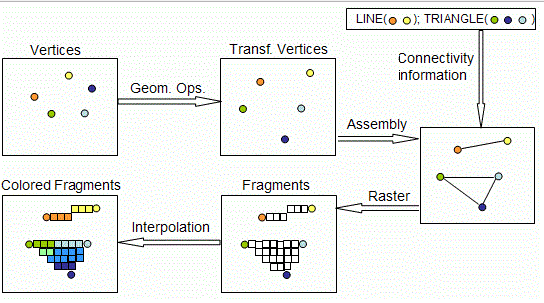
\includegraphics[width=.9\linewidth]{OpenGLPipeline1.png}
				\caption{OpenGL 渲染管线}
			\end{figure}	
			
				
		
	\section{着色器}
		\subsection{程序组成}
			在OpenGL程序中\textbf{使用着色器}一般需要依次执行以下步骤:
			\begin{enumerate}[itemindent = 1em]
				\item 顶点着色程序的源代码和片段着色程序的源代码分别写入到一个文件里(或字符数组)里面,一般顶点着色器源码文件后缀为\textbf{.vert},片段着色器源码文件后缀为\textbf{.frag}
				\item \textbf{使用glCreateshader()}分别创建一个顶点着色器对象和一个片段着色器对象
				\item \textbf{使用glShaderSource()}分别将顶点/片段着色程序的源代码字符数组绑定到顶点/片段着色器对象上
				\item \textbf{使用glCompileShader()}分别编译顶点着色器和片段着色器对象(最好检查一下编译的成功与否)
				\item \textbf{使用glCreaterProgram()}创建一个着色程序对象
				\item \textbf{使用glAttachShader()}将顶点和片段着色器对象附件到需要着色的程序对象上
				\item \textbf{使用glLinkProgram()}分别将顶点和片段着色器和着色程序执行链接生成一个可执行程序(最好检查一下链接的成功与否)
				\item \textbf{使用glUseProgram()}将OpenGL渲染管道切换到着色器模式,并使用当前的着色器进行渲染
			\end{enumerate}	
		
			\textbf{整体流程}如下所示:
			\begin{figure}[htbp]
				\centering
				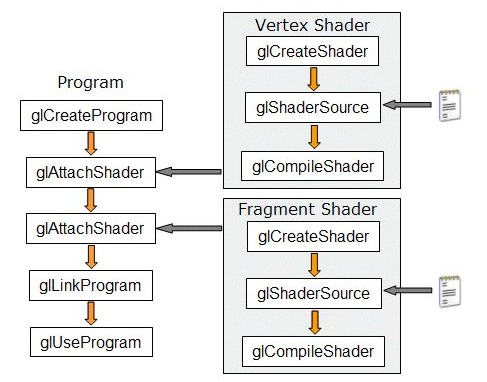
\includegraphics[width = 12cm, height = 6cm]{GLSLProcess.png}
				\caption{GLSL 流程}
				\label{GLSL}
			\end{figure}
			
			\begin{itemize}[itemindent = 1em]
				\item 准备\textbf{原始顶点数据}
				\item 准备\textbf{着色器代码}
				\item \textbf{创建着色器对象}
				\item \textbf{创建着色器程序对象}
				\item \textbf{链接着色器程序对象与着色器对象}
				\item \textbf{在程序中使用着色器}
			\end{itemize}
			
		
		\subsection{数据类型}
		
		
		\subsection{输入输出}
		
		
		\subsection{Uniform}
		
		
		\subsection{自定义属性}
		
		
		\subsection{从文件中读取}		
		
		
		
		
		
		
		

	\section{纹理}
		\subsection{纹理坐标}
			为了能够把纹理映射(Map)到三角形上,我们需要指定三角形的每个顶点各自对应纹理的哪个部分。\textbf{这样每个顶点就会关联着一个纹理坐标(Texture Coordinate),用来标明该从纹理图像的哪个部分采样}(译注:采集片段(\textit{单个像素})颜色)\textbf{。之后在图形的其它片段上进行片段}(\textit{像素})\textbf{插值}(Fragment Interpolation)。
			
			纹理坐标在x和y轴上,\textbf{范围为0到1之间}(注意我们使用的是2D纹理图像)。使用纹理坐标获取纹理颜色叫做采样(Sampling)。纹理坐标起始于(0, 0),也就是纹理图片的左下角,终始于(1, 1),即纹理图片的右上角。下面的图片展示了我们是如何把纹理坐标映射到三角形上的。
			
			\begin{figure}[H]
				\centering
				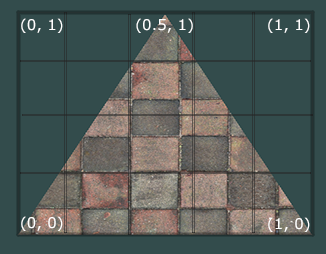
\includegraphics[width=.7\linewidth]{tex_coords}
			\end{figure}
			
			为三角形指定了3个纹理坐标点。如上图所示,我们希望三角形的左下角对应纹理的左下角,因此我们把三角形左下角顶点的纹理坐标设置为(0, 0);三角形的上顶点对应于图片的上中位置所以我们把它的纹理坐标设置为(0.5, 1.0);同理右下方的顶点设置为(1, 0)。\textbf{只要给顶点着色器传递这三个纹理坐标就行了,接下来它们会被传片段着色器中,它会为每个片段进行纹理坐标的插值}。
			
			纹理坐标看起来就像这样:
			\begin{lstlisting}
	float texCoords[] = {
	    0.0f, 0.0f, // 左下角
	    1.0f, 0.0f, // 右下角
	    0.5f, 1.0f // 上中
	};		
			\end{lstlisting}
			
			
		\subsection{环绕模式}
			纹理坐标的范围通常是从(0, 0)到(1, 1),把纹理坐标设置在范围之外会发生什么?OpenGL默认的行为是\textbf{重复这个纹理图像}(我们基本上忽略浮点纹理坐标的整数部分),但OpenGL提供了更多的选择:
			
			\begin{itemize}
				\item \verb|GL_REPEAT|:	对纹理的默认行为。重复纹理图像。
				\item \verb|GL_MIRRORED_REPEAT|:	和\verb|GL_REPEAT|一样,但每次重复图片是镜像放置的。
				\item \verb|GL_CLAMP_TO_EDGE|:	纹理坐标会被约束在0到1之间,超出的部分会重复纹理坐标的边缘,产生一种边缘被拉伸的效果。
				\item \verb|GL_CLAMP_TO_BORDER|:	超出的坐标为用户指定的边缘颜色。
			\end{itemize}
			
			\begin{figure}[H]
				\centering
				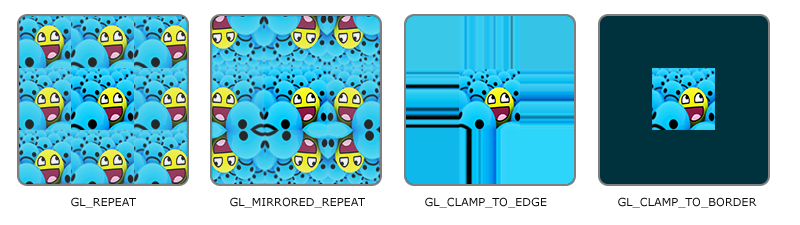
\includegraphics[width=.95\linewidth]{texture_wrapping}
			\end{figure}
			
			每个选项都可以使用\verb|glTexParameter*()函数|对单独的一个坐标轴设置(s、t(如果是使用3D纹理那么还有一个r), 它们和x、y、z是等价的).
			
			\begin{lstlisting}
	glTexParameteri(GL_TEXTURE_2D, GL_TEXTURE_WRAP_S, GL_MIRRORED_REPEAT);
	glTexParameteri(GL_TEXTURE_2D, GL_TEXTURE_WRAP_T, GL_MIRRORED_REPEAT);
			\end{lstlisting}
			
			如果我们选择\verb|GL_CLAMP_TO_BORDER|选项,我们还需要指定一个边缘的颜色。这需要使用 \verb|glTexParameter()函数| 的\textit{fv后缀形式},用\verb|GL_TEXTURE_BORDER_COLOR|作为它的选项,并且\textbf{传递一个float数组作为边缘的颜色值}:
			\begin{lstlisting}
	float borderColor[] = { 1.0f, 1.0f, 0.0f, 1.0f };
	glTexParameterfv(GL_TEXTURE_2D, GL_TEXTURE_BORDER_COLOR, borderColor);
			\end{lstlisting}
			
		
		\subsection{纹理过滤}
			对纹理进行\textit{放大或者缩小}的过程叫做纹理过滤, 纹理过滤有很多个选项,现在只讨论最重要的两种:
			
			\paragraph{临近过滤}
				\verb|GL_NEAREST|(也叫邻近过滤,Nearest Neighbor Filtering)是OpenGL\textit{默认的纹理过滤方式}。当设置为\verb|GL_NEAREST|的时候,OpenGL会\textbf{选择中心点最接近纹理坐标的那个像素}。下图中你可以看到四个像素,加号代表纹理坐标。左上角那个纹理像素的中心距离纹理坐标最近,所以它会被选择为样本颜色:
				
				\begin{figure}[H]
					\centering
					
\includegraphics[width=.5\linewidth]{filter_nearest}
				\end{figure}
			
			\paragraph{线性过滤}
				\verb|GL_LINEAR|(也叫线性过滤,(Bi)linear Filtering)它会\textbf{基于纹理坐标附近的纹理像素,计算出一个插值,近似出这些纹理像素之间的颜色}。一个纹理像素的中心距离纹理坐标越近,那么这个纹理像素的颜色对最终的样本颜色的贡献越大。下图中你可以看到返回的颜色是邻近像素的混合色:
				\begin{figure}[H]
					\centering
					
\includegraphics[width=.5\linewidth]{filter_linear}
				\end{figure}			
		
			
			\paragraph{应用与比较}
				当进行\textbf{放大(Magnify)和缩小(Minify)}操作的时候可以\textbf{设置纹理过滤}的选项,比如你可以在纹理被缩小的时候使用邻近过滤,被放大时使用线性过滤。我们需要使用\textbf{glTexParameter*()函数}为放大和缩小指定过滤方式。
				
				\begin{lstlisting}
	glTexParameteri(GL_TEXTURE_2D, GL_TEXTURE_MIN_FILTER, GL_NEAREST);
	glTexParameteri(GL_TEXTURE_2D, GL_TEXTURE_MAG_FILTER, GL_LINEAR);			
				\end{lstlisting}
				
				\begin{figure}[H]
					\centering
					
\includegraphics[width=.9\linewidth]{texture_filtering}
					\caption{临近过滤与线性过滤比较}
				\end{figure}
			
			
		\subsection{多级纹理-mipmap}
			想象一下,假设我们有一个包含着上千物体的大房间,每个物体上都有纹理。有些物体会很远,但其纹理会拥有与近处物体同样高的分辨率。由于远处的物体可能只产生很少的片段,OpenGL从高分辨率纹理中为这些片段获取正确的颜色值就很困难,因为它需要对一个跨过纹理很大部分的片段只拾取一个纹理颜色。在小物体上这会\textbf{产生不真实的感觉},更不用说对它们使用\textbf{高分辨率纹理浪费内存的问题}了。		
			
			OpenGL使用一种叫做多级渐远纹理(Mipmap)的概念来解决这个问题,它简单来说就是一系列的纹理图像,后一个纹理图像是前一个的二分之一。多级渐远纹理背后的理念很简单:距观察者的距离超过一定的阈值,OpenGL会使用不同的多级渐远纹理,即最适合物体的距离的那个。由于距离远,解析度不高也不会被用户注意到。同时,多级渐远纹理另一加分之处是它的性能非常好。
			
			\begin{figure}[H]
				\centering
				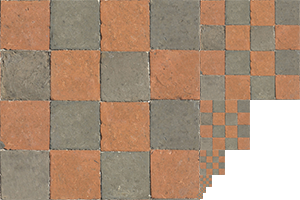
\includegraphics[width=.7\linewidth]{mipmaps}
			\end{figure}
			
			OpenGL有一个glGenerateMipmaps函数,在创建完一个纹理后调用它OpenGL就会创建该纹理的mipmap.
			
			在渲染中切换多级渐远纹理级别(Level)时,OpenGL在两个不同级别的多级渐远纹理层之间会产生不真实的生硬边界。就像普通的纹理过滤一样,切换多级渐远纹理级别时你也可以在两个不同多级渐远纹理级别之间使用NEAREST和LINEAR过滤。
			
			为了指定不同多级渐远纹理级别之间的过滤方式,你可以使用下面四个选项中的一个代替原有的过滤方式:
			\begin{itemize}
				\item \verb|GL_NEAREST_MIPMAP_NEAREST|	使用最邻近的多级渐远纹理来匹配像素大小,并使用邻近插值进行纹理采样
				\item \verb|GL_NEAREST_MIPMAP_LINEAR|	在两个最匹配像素大小的多级渐远纹理之间进行线性插值,使用邻近插值进行采样
				\item \verb|GL_LINEAR_MIPMAP_NEAREST|	使用最邻近的多级渐远纹理级别,并使用线性插值进行采样
				\item \verb|GL_LINEAR_MIPMAP_LINEAR|	在两个邻近的多级渐远纹理之间使用线性插值,并使用线性插值进行采样
			\end{itemize}
			
			就像纹理过滤一样,我们可以使用glTexParameteri将过滤方式设置为前面四种提到的方法之一:
			\begin{lstlisting}
	glTexParameteri(GL_TEXTURE_2D, GL_TEXTURE_MIN_FILTER, GL_LINEAR_MIPMAP_LINEAR);
	glTexParameteri(GL_TEXTURE_2D, GL_TEXTURE_MAG_FILTER, GL_LINEAR);				
			\end{lstlisting}
			
			
			多级渐远纹理\textbf{主要是使用在纹理被缩小的情况下的}:纹理放大不会使用多级渐远纹理,为放大过滤设置多级渐远纹理的选项会产生一个\verb|GL_INVALID_ENUM|错误代码。
			
		\subsection{纹理压缩格式}
			etc1、etc2、dds
		
		
		\subsection{应用}
			分为5个步骤,加载图片源、创建纹理、设置纹理属性、顶点着色器传递纹理坐标、片元着色器使用纹理坐标取色。
			
			\paragraph{加载图片源-SOIL}
				使用SOIL 库(Simple OpenGL Image Library)
				
				\begin{lstlisting}
	#include <SOIL.h>
	int width, height;
	unsigned char* image = SOIL_load_image("container.jpg", &width, &height, 0, SOIL_LOAD_RGB);			
				\end{lstlisting}
				
				函数首先需要输入图片文件的\textbf{路径}。然后需要两个int指针作为第二个和第三个参数,SOIL会分别返回图片的宽度和高度到其中。后面我们在生成纹理的时候会用图像的宽度和高度。第四个参数指定图片的通道(Channel)数量,但是这里我们只需留为0。最后一个参数告诉SOIL如何来加载图片:我们只关注图片的RGB值。结果会储存为一个很大的char/byte数组。
			
			\paragraph{创建纹理-设置纹理属性}
				和之前生成的OpenGL对象一样,纹理也是使用ID引用的。
				
				\begin{lstlisting}
	GLuint texture;
	glGenTextures(1, &texture);		
	glBindTexture(GL_TEXTURE_2D, texture);	
	// 为当前绑定的纹理对象设置环绕、过滤方式
	...
	// 加载并生成纹理
	glTexImage2D(GL_TEXTURE_2D, 0, GL_RGB, width, height, 0, GL_RGB, GL_UNSIGNED_BYTE, image);
	glGenerateMipmap(GL_TEXTURE_2D);	
	SOIL_free_image_data(image);
	glBindTexture(GL_TEXTURE_2D, 0);
				\end{lstlisting}

			\paragraph{顶点着色器传递纹理坐标}
				
				通过VBO 顶点属性传递。
				
				\begin{lstlisting}
	#version 330 core
	layout (location = 0) in vec3 position;
	layout (location = 1) in vec3 color;
	layout (location = 2) in vec2 texCoord;
	
	out vec3 ourColor;
	out vec2 TexCoord;
	
	void main()
	{
	    gl_Position = vec4(position, 1.0f);
	    ourColor = color;
	    TexCoord = texCoord;
	}				
				\end{lstlisting}
				
			
			\paragraph{片元着色器使用uv坐标取色}
				
				通过uniform 将纹理传递过来,通过顶点着色器将纹理坐标传过来,然后取出当前UV坐标点的像素颜色。
			
				\begin{lstlisting}
	#version 330 core
	in vec3 ourColor;
	in vec2 TexCoord;
	
	out vec4 color;
	
	uniform sampler2D ourTexture;
	
	void main()
	{
	    color = texture(ourTexture, TexCoord);
	}				
				\end{lstlisting}
			
			
			\paragraph{纹理混合}
				两张或多张(至多16) 以某种方式混合
				
				\begin{lstlisting}
	#version 330 core
	...
	
	uniform sampler2D ourTexture1;
	uniform sampler2D ourTexture2;
	
	void main()
	{
	    color = mix(texture(ourTexture1, TexCoord), texture(ourTexture2, TexCoord), 0.2);
	}				
				\end{lstlisting}


\chapter{三大变换}
	从这个教程开始我们开始研究各种各样的图形变换,\textbf{图形变换就可以让一个3d物体在屏幕中变换的的时候看上去保持有深度的错觉},也就是立体的投影效果。
	
	\textbf{实现}立体效果的\textbf{方法是}使用一个\textbf{经过多次相乘的变换矩阵}得到的\textbf{最终变换矩阵}来\textbf{和顶点的位置再相乘},\textit{这样得到3d物体的一个多次变换后的最终复合变换效果}。
	
	\section{平移}
		参考文献:\url{https://blog.csdn.net/cordova/article/details/52541902}
		
		为了实现平移转换\textbf{所以矩阵是4*4的}
		
		
		这里我们先看一下平移变换,使一个物体沿着一个任意长度任意方向的向量平移,比如说让一个三角形从左边移动到右边:
			\begin{figure}[h]
				\centering
				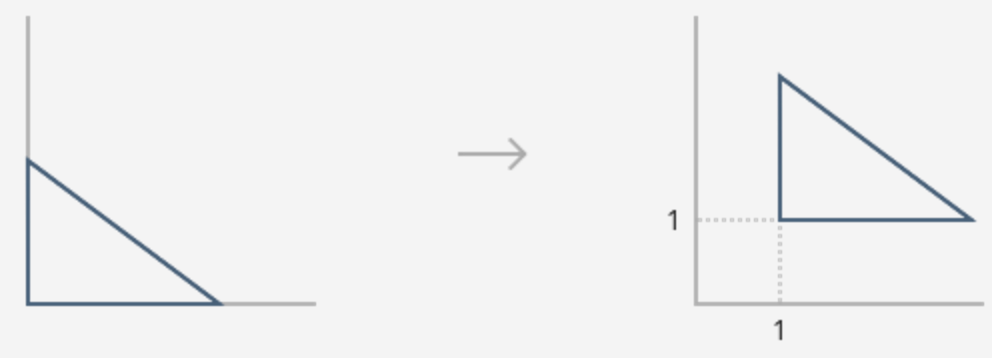
\includegraphics[width=.7\linewidth]{transfer.png}
				\caption{平移示例}
			\end{figure}

		在之前顶点着色器知识的基础上我们可以想到实现平移的一种办法是设置一个偏移向量(这里就是- 1了),并把这个便宜向量定义成一致变量然后传递给shader让每一个顶点按照那个偏移向量移动即可。
		
		但这样就\textit{打破}\textbf{通过乘以一个经过多个变换矩阵相乘得到的复合变换矩阵来进行复合变换}\textit{的统一性了}。
		 
		统一的说,我们是想找到这样一个矩阵,对于给定的\verb|点P(x,y,z)|和平移向量$V(v1,v2,v3)$,能够使 $M * P = P1(x+v1, y+v2, z+v3) $,简单地说就是\verb|矩阵M将P转换成了P+V|。在结果向量\verb|P1|中我们可以看到每个分量是\verb|P|和\verb|V|每个分量对应相加的和,结果向量P1的+号左侧来自P本身,对于得到P本身的向量应该这样: 
		\verb|I * P = P(x,y,z)| 。所以我们应该从得到本身开始来调整变换矩阵得到结果矩阵右侧相加结果(…+V1, …+V2, …+V3)的最终变换矩阵。首先自身变换矩阵的样子如下:
			\begin{equation}
			 \left(
			\begin{array}{ccc}
			1 & 0 & 0\\
			
			0 & 1 & 0\\
			
			0 & 0 & 1\\
			\end{array}
			\right)
			\left(
			\begin{array}{c}
				X\\ 
				Y\\
				Z 
			\end{array}	
			\right) 
			=
			\left(
				\begin{array}{c}
				X\\ 
				Y\\
				Z 
				\end{array}	
			\right)
		\end{equation}
		
		我们想修改这个自身变换矩阵使结果变成这样子:
			$$
				\left(
				\begin{array}{c}
				X+V_1\\ 
				Y+V_2\\
				Z+V_3 
				\end{array}	
				\right)
			$$
		
		如果我们坚持用$3\times3$矩阵好像不可能得到想要的结果,但如果改成$4\times4$矩阵我可以这样得到想要的结果:
			\begin{equation}
			\left(
			\begin{array}{cccc}
			1 & 0 & 0& V_1\\
			
			0 & 1 & 0& V_2\\
			
			0 & 0 & 1& V_3\\
			
			0 & 0 & 0& 1\\
			\end{array}
			\right)
			\left(
			\begin{array}{c}
			X\\ 
			Y\\
			Z\\
			1 
			\end{array}	
			\right) 
			=
			\left(
			\begin{array}{c}
			X+V_1\\ 
			Y+V_2\\
			Z+V_3\\
			1 
			\end{array}	
			\right)
			\end{equation}
		
		这样使用一个4维向量表示一个3维向量叫做\textbf{齐次坐标},这在3d图形学中很常用也很有用,第四个分量称作\verb|“w”|。事实上,我们之前教程中看到的内部shader符号变量\verb|gl_Position|就是一个4维向量,第四个分量\verb|“w”|在从3d到2d的投影变换中起着关键作用。通常对于表示点的矩阵会让\verb|w=1|,而对于表示向量的矩阵会让\verb|w=0|,\textbf{因为点可以被做变换而向量不可以},你可以改变一个向量的长度和方向,但是长度和方向一样的所有向量都是相等的,不管他们的起点在哪里,所以我们可以把所有的向量起点放到原点来看。对于向量设置\verb|w=0|然后乘以\textbf{变换矩阵}会得到\textbf{和自身一样的向量}。
		
	\section{旋转}
		参考文献:\url{https://blog.csdn.net/cordova/article/details/52558133}
		
		旋转变换将总是改变位置的其中两个坐标,第三个坐标保持不变,这意味着旋转的路径会保持在其中一个平面上:XY平面(绕Z轴旋转),YZ平面(绕X轴旋转)和XZ平面(绕Y轴旋转)。也有一些复杂的旋转变换允许图形绕着任意向量旋转,但在我们这个阶段还不需要。
		
		让我们从普遍统一的角度来定义这个问题。看下面这个图:
			\begin{figure}[h]
				\centering
				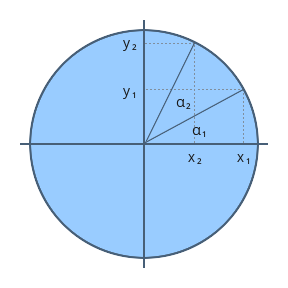
\includegraphics[scale = 0.7]{rotate.png}
				\caption{旋转示例}
			\end{figure}
		
		我们想从(x1,y1)沿着圆移动到(x2,y2),换句话说就是将点(x1,y1)旋转a2角度。假设圆的半径是1,那有下面的式子:
		\begin{equation}
			\begin{cases}
				x_1 = cos(\alpha_1)\\
				y_1 = sin(\alpha_1)\\
				x_2 = cos(\alpha_1 + \alpha_2)\\
				y_2 = sin(\alpha_1 + \alpha_2)
			\end{cases}
		\end{equation}
		
		我们用下面的三角函数变换公式来推导x2和y2的表达式:
		$$
			\begin{cases}
				cos(\alpha_1 + \alpha_2) = cos(\alpha_1)\cdot cos(\alpha_2) - sin(\alpha_1)\cdot sin(\alpha_2)\\
				sin(\alpha_1 + \alpha_2) = sin(\alpha_1)\cdot cos(\alpha_2) + cos(\alpha_1)\cdot sin(\alpha_2)
			\end{cases}
		$$
		
		上式等价于
		$$
		\begin{cases}
			x_2 = x_1\cdot cos(\alpha_2) - y_1\cdot sin(\alpha_2)\\
			y_2 = y_1\cdot cos(\alpha_2) + x_1\cdot sin(\alpha_2)
		\end{cases}
		$$
		
		
		再上面的图中我们看的是XY平面,Z轴指向纸面。X和Y放在4维矩阵里面的的话那么上面的公式可以写成下面的矩阵形式(不影响Z和W分量):
		
		\begin{equation}
		\left(
		\begin{array}{cccc}
		cos(\alpha_2) & -sin(\alpha_2) & 0& V_1\\
		
		sin(\alpha_2) & cos(\alpha_2) & 0& V_2\\
		
		0 & 0 & 1& V_3\\
		
		0 & 0 & 0& 1\\
		\end{array}
		\right)
		\left(
		\begin{array}{c}
		X\\ 
		Y\\
		Z\\
		1 
		\end{array}	
		\right) 
		=
		\left(
		\begin{array}{c}
		x_1\cdot cos(\alpha_2) - y_1\cdot sin(\alpha_2)\\ 
		y_1\cdot cos(\alpha_2) + x_1\cdot sin(\alpha_2)\\
		Z+V_3\\
		1 
		\end{array}	
		\right)
		\end{equation}
	\section{缩放}
		参考文献:\url{https://blog.csdn.net/cordova/article/details/52558804}

		缩放变换非常简单,它的目的是增大或者缩小物体的尺寸。比如你想使用同一个模型来制作很多不同的物体(大小不一的树组成的树林,用的同一个模型),或者你想按照比例让物体和现实世界尺寸一致。在上面的情形中你就需要在三个坐标轴上同等缩放顶点的位置。当然,有时也希望物体只在一个轴上或者两个轴上缩放使模型更薄、更瘦或者更高等等。
		
		进行缩放变换其实很简单。我们从最开始的原变换矩阵来看,回忆平移变换矩阵的样子,我们保持结果矩阵中V1,V2和V3保持原样的办法是让变换矩阵主对角线上的值都为’1’,这样原向量一次都和1相乘之后依然保持不变,各分量之间互不影响。所以,这里的缩放变换,只要把那些‘1’换成我们想缩放的值,原向量各分量分别乘以这些值之后就会在相应坐标轴上进行相应的缩放了,值大于1则放大,值小于1则缩小。
		
		\begin{figure}[h]
			\centering
			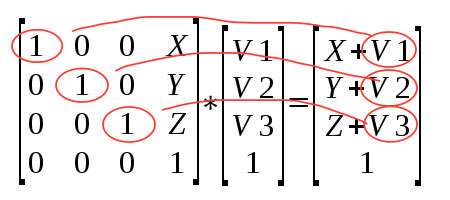
\includegraphics[scale = 0.57]{scale_1.png}
			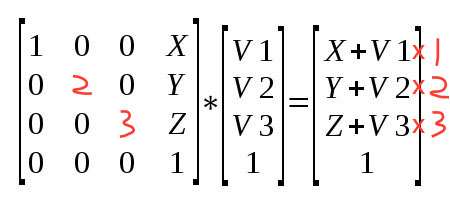
\includegraphics[scale = 0.57]{scale_2.png}
			\caption{缩放示例}
		\end{figure}

\chapter{四大变换}
参考文献:\url{http://blog.csdn.net/lyx2007825/article/details/8792475}

\verb|--|:\url{https://blog.csdn.net/u012501459/article/details/12945147}

\verb|数学变换过程:|\url{https://blog.csdn.net/wangdingqiaoit/article/details/51594408}

	\section{坐标变化全过程演示}
		OpenGL中的坐标处理过程包括\textbf{模型变换}、\textbf{照像机变换}、\textbf{投影变换}、\textbf{视口变换}等过程,如下图所示:
		
		\begin{figure}[htbp]
			\centering
			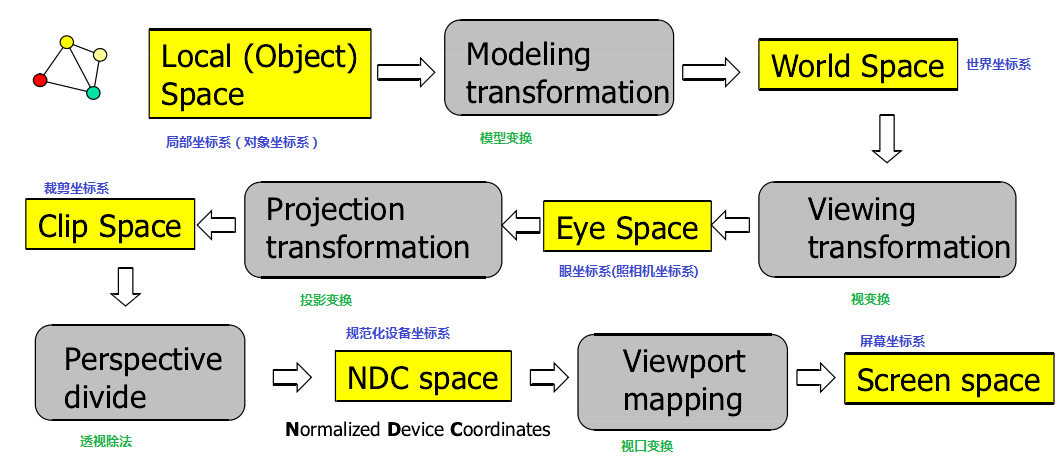
\includegraphics[scale = 0.57]{transferAll.png}
			\caption{转化流程}
		\end{figure}
		
		在上面的图中,注意,OpenGL只定义了\textit{裁剪坐标系、规范化设备坐标系和屏幕坐标系},而\textbf{局部坐标系(模型坐标系)、世界坐标系和照相机坐标系}都是为了方便用户设计而自定义的坐标系,它们的关系如下图所示
		
		\begin{figure}[htbp]
			\centering
			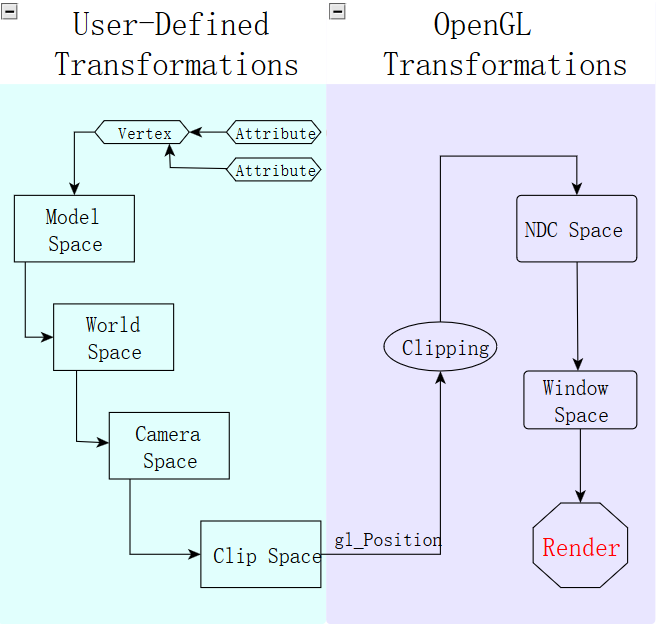
\includegraphics[scale = 0.9]{transferAll2.png}
			\caption{转化流程2}
		\end{figure}
		
		图中左边的过程包括模型变换、视变换,投影变换,这些变换可以由用户根据需要自行指定,这些内容在顶点着色器中完成;而图中右边的两个步骤,包括透视除法、视口变换,这两个步骤是OpenGL自动执行的,在顶点着色器处理后的阶段完成。
		
	\section{模型变换(世界变换)}
			\subparagraph{包含}:所有单位模型的变换,为了能够在世界坐标系中正确的显式相对位置。如图\ref{mxzh}
				\begin{figure}[htbp]
					\centering
					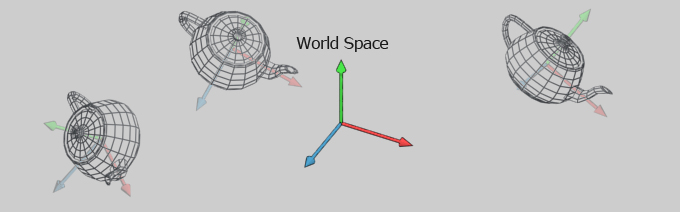
\includegraphics[scale = 0.7]{transferModel.png}
					\caption{模型转换过程}
					\label{mxzh}
				\end{figure}
			
			\subparagraph{顺序}:\verb|缩放–>旋转—>平移|
		
			\subparagraph{数学}->\verb|变换矩阵*位置坐标|,如公式\ref{model transform}
					\begin{equation}\label{model transform}
					\left(
					\begin{array}{cccc}
					1 & 0 & 0& V_1\\
					
					0 & 1 & 0& V_2\\
					
					0 & 0 & 1& V_3\\
					
					0 & 0 & 0& 1\\
					\end{array}
					\right)
					\left(
					\begin{array}{c}
					X\\ 
					Y\\
					Z\\
					1 
					\end{array}	
					\right) 
					=
					\left(
					\begin{array}{c}
					X+V_1\\ 
					Y+V_2\\
					Z+V_3\\
					1 
					\end{array}	
					\right)
					\end{equation}
		
		
			利用GLM数学库实现模型变换,例如平移变换示例代码为:
			\begin{lstlisting}
	glm::mat4 model; // 构造单位矩阵
	model = glm::translate(model, glm::vec3(0.0f, 0.0f,-0.5f));
			\end{lstlisting}
			
	\section{摄像机变换}
			数学变换参考文献:\url{https://blog.csdn.net/wangdingqiaoit/article/details/51570001}
			
			\subparagraph{包含}:相机坐标系中的坐标,就是从相机的角度来解释世界坐标系中位置。如
				\begin{figure}[htbp]
					\centering
					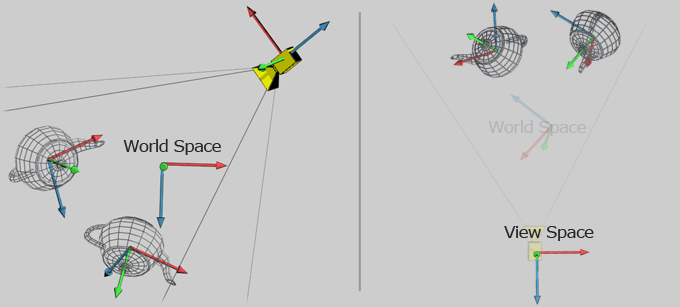
\includegraphics[scale = 0.7]{transferEye.png}
					\caption{摄像机转换过程}
				\end{figure}
			
			\subparagraph{数学}:OpenGL中相机始终位于原点,指向-Z轴,而以相反的方式来调整场景中物体,从而达到相同的观察效果。例如要观察-z轴方向的一个立方体的右侧面,可以有两种方式:
				\begin{itemize}[itemindent = 1em]
					\item \textbf{立方体不动},让相机绕着+y轴,旋转+90度,此时相机镜头朝向立方体的右侧面,实现目的。完成这一旋转的矩阵记作$R_y(\frac{\pi}{2})$
					\item \textbf{相机不动},让立方体绕着+y轴,旋转-90度,此时也能实现同样的目的。注意这时相机没有转动。完成这一旋转的矩阵记作$R_y(-\frac{\pi}{2})$
				\end{itemize}
				
				\textbf{OpenGL中采用方式2的观点来解释视变换。}例如下面\ref{sxweizhi}的图表示了假想的相机:
				\begin{figure}[htbp]
					\centering
					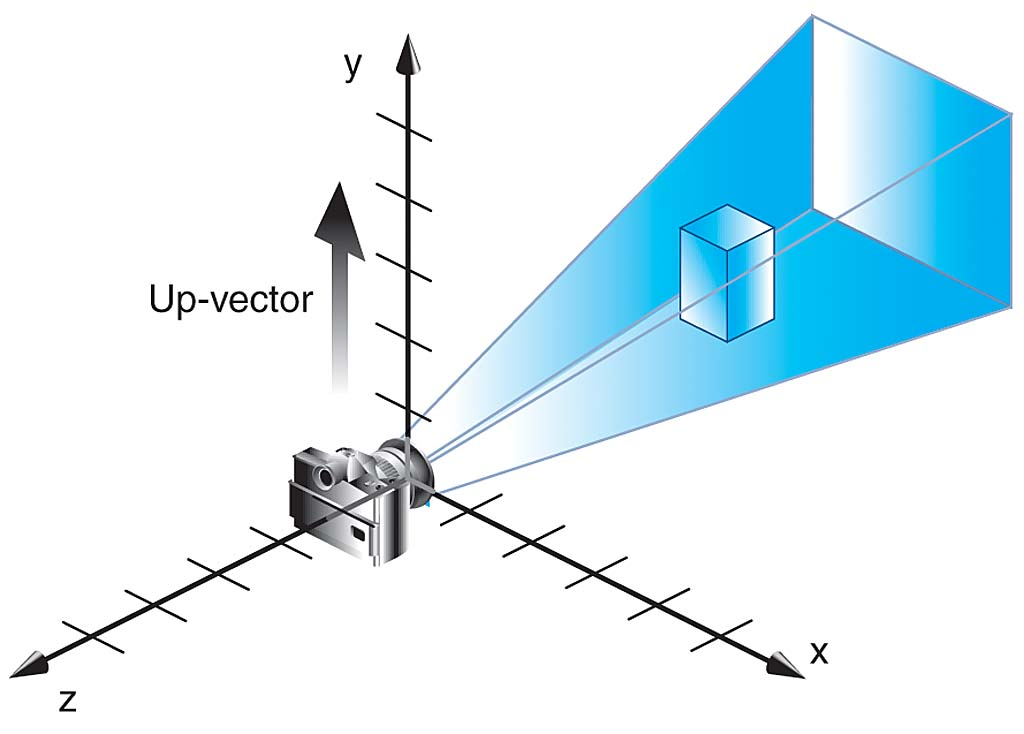
\includegraphics[scale = 0.4]{Eye.png}
					\caption{openGL摄像机位置}
					\label{sxweizhi}
				\end{figure}	
				
				再举一个例子,比如,\textit{一个物体中心位于原点,照相机也位于初始位置原点,方向指向-Z轴}。\textbf{为了对物体的+Z面成像},那么必须将照相机从原点移走,如果照相机仍然指向-Z轴,需要将照相机沿着+Z轴方向后退。假若照相机不移动,我们可以通过将物体沿着-Z轴后退d个单位,则变换矩阵为:
					$$
					Matrix = 
					\left(
					\begin{array}{cccc}
					1 & 0 & 0& 0\\
					
					0 & 1 & 0& 0\\
					
					0 & 0 & 1& -d\\
					
					0 & 0 & 0& 1\\
					\end{array}
					\right)
					$$
					
			进一步说明这里相对的概念,对这个概念不感兴趣的可以跳过。默认时相机位于(0,0,0),指向-z轴,相当于调用了:
			\begin{lstlisting}
	glm::lookAt(glm::vec(0.0f,0.0f,0.0f),
		glm::vec3(0.0f, 0.0f, -1.0f),
		glm::vec3(0.0f, 1.0f, 0.0f));
			\end{lstlisting}
			得到是单位矩阵,\textbf{这是相机的默认情况}。
			
			\textbf{上述第一种方式},相机绕着+y轴旋转90度,相机指向-x轴,则等价于调用变为:
			\begin{lstlisting}
	glm::mat4 view =glm::lookAt(glm::vec(0.0f,0.0f,0.0f),
		glm::vec3(-1.0f, 0.0f, 0.0f),
		glm::vec3(0.0f, 1.0f, 0.0f));
			\end{lstlisting}
			得到的视变换矩阵为:
				$$
				Matrix = 
				\left(
				\begin{array}{cccc}
				0 & 0 & -1& 0\\
				
				0 & 1 & 0& 0\\
				
				1 & 0 & 0& 0\\
				
				0 & 0 & 0& 1\\
				\end{array}
				\right)
				$$
			
			\textbf{上述第二种方式},通过立方体绕着+y轴旋转-90度,则得到的矩阵M,相当于:
				\begin{lstlisting}
	glm::mat4 model = glm::rotate(glm::mat4(1.0), glm::radians(-90.0f), glm::vec3(0.0, 1.0, 0.0));
				\end{lstlisting}
				
			\textbf{这里得到的矩阵M和上面的矩阵view是相同的},可以自行验证下。 
			\textit{也就是说,通过旋转相机+y轴90度,和旋转立方体+y轴-90度,最终计算得到的}\textbf{矩阵相同}。调整相机来得到观察效果,可以通过相应的方式来调整物体达到相同的效果。在OpenGL中并不存在真正的相机,这只是一个虚构的概念。
			
			\subparagraph{计算变换矩阵}
				相机坐标系由相机位置eye和UVN基向量(或者说由forward, side ,up)构成,如下图\ref{shexiang}所示:
				\begin{figure}[htbp]
					\centering
					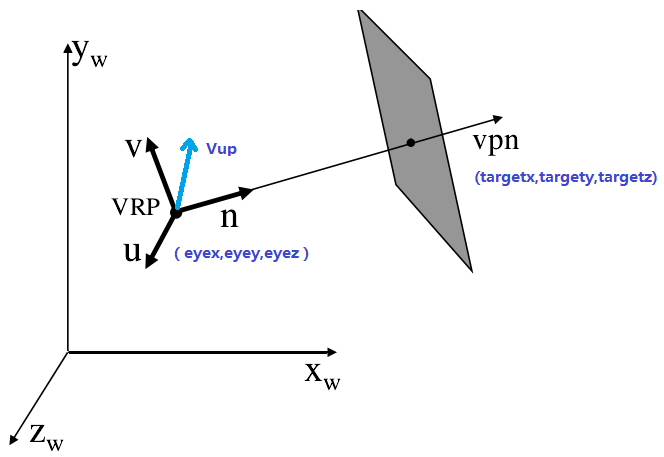
\includegraphics[scale = 0.7]{EyeTrans.png}
					\caption{摄像机-物体图例}
					\label{shexiang}
				\end{figure}
				
				各个参数的含义如下:
				\begin{itemize}[itemindent = 1em]
					\item \textbf{相机位置 }也称为观察参考点 (View Reference Point) 在世界坐标系下指定相机的位置\textbf{eye}。
					\item \textbf{相机镜头方向},由相机位置和相机指向的目标(target)位置计算出,$forwrad=(target−eye)$。
					\item \textbf{相机顶部正朝向}: View Up Vector 确定在相机哪个方向是向上的,一般取(0, 1, 0)。
				\end{itemize}
				上面的图简化为图\ref{shexiangjie2}: 
				\begin{figure}[htbp]
					\centering
					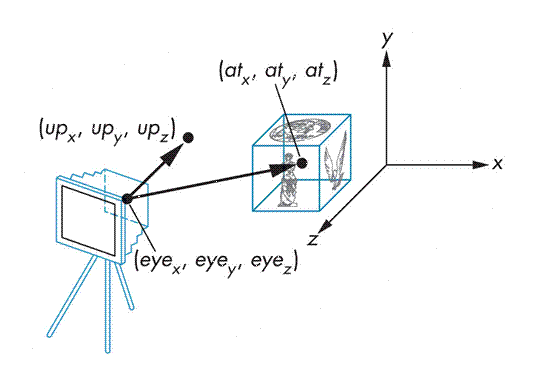
\includegraphics[scale = 0.7]{EyeTrans2.png}
					\caption{摄像机-物体图例2}
					\label{shexiangjie2}
				\end{figure}
				
				在使用过程中,我们是要指定的参数即为\textbf{相机位置(eye)},\textbf{相机指向的目标位置(target)}和\textbf{viewUp vector}三个参数。 
				
				\begin{enumerate}[itemindent = 1em]
					\item 首选\textbf{计算相机镜头方向}:$forwrad=(target−eye)$,并完成标准化$\frac{forward}{|forward|}$
					\item 根据view-up vector和forward\textbf{确定相机的side向量}:
						$$viewUp' = \dfrac{viewUp}{||viewUp||}$$
						$$side = cross(forward, viewUp')$$
					\item 根据forward和side\textbf{计算up向量}: 
						$$up=cross(side,forward)$$
				\end{enumerate}
				
				这样\textbf{eye位置,以及forward、side、up三个基向量构成一个新的坐标系},注意这个坐标系是一个\textbf{左手坐标系},因此在实际使用中,\textbf{需要对forward进行一个翻转,利用-forward、side、up和eye来构成一个右手坐标系}。
				
				从坐标和变换一节,了解到,要实现不同坐标系之间的坐标转换,需要求取一个变换矩阵。而这个矩阵就是一个坐标系A中的原点和基在另一个坐标系B下的表示。 
				
				我们将相机坐标系的原点和基,使用世界坐标系表示为(s代表side基向量,u代表up基向量,f代表forward基向量): 
								$$
								CameraWorld =  
								\left(
								\begin{array}{cccc}
								s[0] & u[0] & -f[0]& eye_x\\
								
								s[1] & u[1] & -f[1]& eye_y\\
								
								s[2] & u[2] & -f[2]& eye_z\\
								
								0 & 0 & 0& 1\\
								\end{array}
								\right)
								$$
								
				通过一些列变换求得视变换矩阵为
					$$
					Model_{view} =  
					\left(
					\begin{array}{cccc}
						s[0] & s[1] & s[2]& -dot(s,eye)\\
						
						u[0] & u[1] & u[2]& -dot(u,eye)\\
						
						-f[0] & -f[1] & -f[2]& dot(f,eye)\\
						
						0 & 0 & 0& 1\\
					\end{array}
					\right)
					$$
					
				这种方式对应的计算代码如下:
				\begin{lstlisting}
	// 手动构造LookAt矩阵 方式1
	glm::mat4 computeLookAtMatrix1(glm::vec3 eye, glm::vec3 target, glm::vec3 viewUp)
	{
		glm::vec3 f = glm::normalize(target - eye); // forward vector
		glm::vec3 s = glm::normalize(glm::cross(f, viewUp)); // side vector
		glm::vec3 u = glm::normalize(glm::cross(s, f)); // up vector
		glm::mat4 lookAtMat(
				glm::vec4(s.x, u.x, -f.x, 0.0), // 第一列
				glm::vec4(s.y, u.y, -f.y, 0.0), // 第二列
				glm::vec4(s.z, u.z, -f.z, 0.0), // 第三列
				glm::vec4(-glm::dot(s, eye),
				-glm::dot(u, eye), glm::dot(f, eye), 1.0)  // 第四列
			);
		return lookAtMat;
	}
				\end{lstlisting}
				
				而最终结果则可以表示为
				$$ 	
				\left(
				\begin{array}{c}
				X_{eye}\\ 
				Y_{eye}\\
				Z_{eye}\\
				w_{eye}
				\end{array}	
				\right) 
				=
				Matrix_{view}
				\cdot
				Matrix_{model}
				\cdot
				\left(
				\begin{array}{c}
				X_{obj}\\ 
				Y_{obj}\\
				Z_{obj}\\
				w_{obj}
				\end{array}	
				\right) 
				$$
				
	\section{投影变换}
			数学变换参考文献:\url{https://blog.csdn.net/wangdingqiaoit/article/details/51589825}
			
			\subparagraph{含义}:投影方式决定以何种方式成像,投影方式有很多种,OpenGL中主要使用两种方式,即透视投影(perspective projection)和正交投影( orthographic projection)。
			\begin{itemize}[itemindent = 1em]
				\item \textbf{正交投影}是平行投影的一种特殊情形,正交投影的投影线垂直于观察平面。平行投影的投影线相互平行,投影的结果与原物体的大小相等,因此广泛地应用于工程制图等方面。 
				\item \textbf{透视投影}的投影线相交于一点,因此投影的结果与原物体的实际大小并不一致,而是会近大远小。因此透视投影更接近于真实世界的投影方式。
			\end{itemize}
			两者的示意图如下\ref{tyqb}:
			\begin{figure}[htbp]
				\centering
				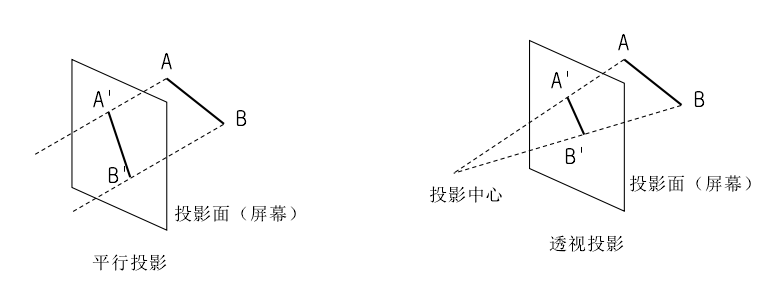
\includegraphics[scale = 0.7]{project.png}
				\caption{投影区别}
				\label{tyqb}
			\end{figure}
			在OpenGL中成像时的效果如下\ref{touyingqubie}所示:
			   \begin{figure}[htbp]
			   	\centering
			   	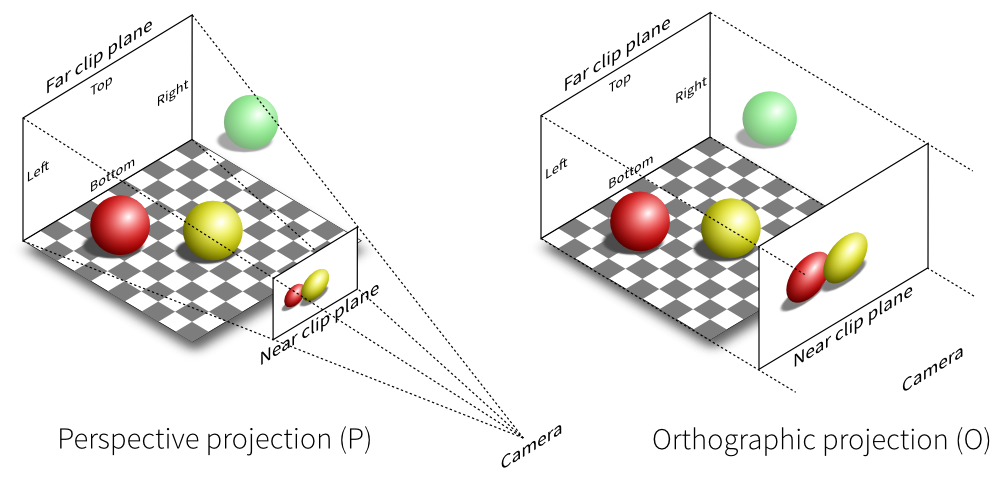
\includegraphics[scale = 0.7]{project2.png}
			   	\caption{openGL投影区别}
			   	\label{touyingqubie}
			   \end{figure}
			上面的图中,红色和黄色球在视见体内,因而呈现在投影平面上,而绿色球在视见体外,没有在投影平面上成像。  注意在相机坐标系下,相机指向$-z$轴,nearVal和farVal表示的剪裁平面分别为:近裁剪平面$z=−nearVal$,以及远裁剪平面$z=−farVal$ 
			
			在openGL 实现如下:
			
			使用\verb|glOrtho(xleft, xright, ybottom, ytop, znear, zfar);|或者类似API\textbf{指定正交投影},参数意义形象表示为下图\ref{zhengjiao}所示
				\begin{figure}[htbp]
					\centering
					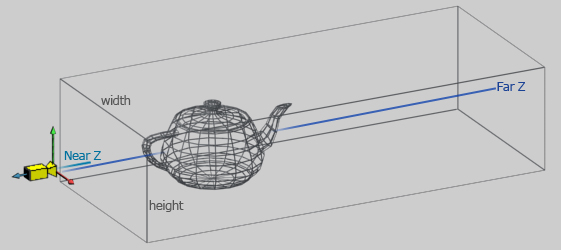
\includegraphics[scale = 0.7]{Ortho.png}
					\caption{openGL正交投影效果}
					\label{zhengjiao}
				\end{figure}
			
			使用\verb|void gluPerspective(...);|或者类似的API指定透视投影的视见体,其参数含义如下图\ref{toushi}所示
				\begin{figure}[htbp]
					\centering
					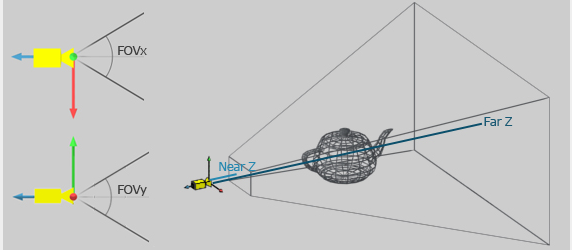
\includegraphics[scale = 0.7]{project3.png}
					\caption{openGL透视投影效果}
					\label{toushi}
				\end{figure}
				
			另外一种经常使用 的方式是\textbf{通过视角(Fov),宽高比(Aspect)来指定透视投影},例如旧版中函数gluPerspective 如图\ref{ts1}:
				\begin{figure}[htbp]
					\centering
					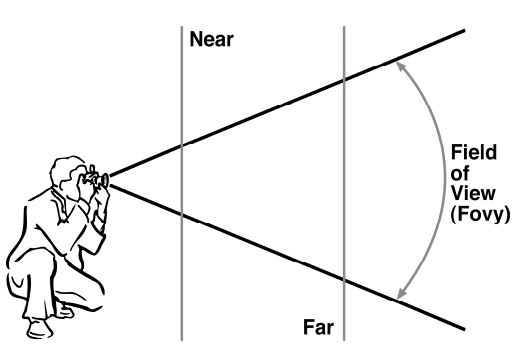
\includegraphics[scale = 0.7]{toushi.png}
					\caption{openGL投影示意}
					\label{ts1}
				\end{figure}
			
			这些参数指定的是一个对称的视见体,如下图\ref{ts2}所示
				\begin{figure}[htbp]
					\centering
					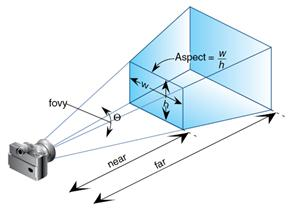
\includegraphics[scale = 1]{toushi2.png}
					\caption{openGL投影示意2}
					\label{ts2}
				\end{figure}
		
			由这些参数,可以得到: 
				\begin{itemize}[itemindent = 1em]
					\item $h=near∗tan(\dfrac{\theta}{2})$
					\item $w=h*Aspect$
					\item $r=−l,r=w$
					\item $t=−b,t=h$
				\end{itemize}
				
			则得到透视投影矩阵为:
				$$
				Model_{project} =  
				\left(
				\begin{array}{cccc}
				\dfrac{cot(\frac{\theta}{2})}{Aspect} & 0 & 0& 0\\
				
				0 & cot(\frac{\theta}{2}) & 0& 0\\
				
				0 & 0 & \dfrac{-(f+n)}{f-n}& \dfrac{-2fn}{f-n}\\
				
				0 & 0 & -1& 0\\
				\end{array}
				\right)
				$$
				
			通过一系列变换,最后的变换矩阵使用如下所示	
				$$ 	
				\left(
				\begin{array}{c}
					X_{clip}\\ 
					Y_{clip}\\
					Z_{clip}\\
					w_{clip}
				\end{array}	
				\right) 
				=
				Matrix_{projection}
				\cdot
				\left(
				\begin{array}{c}
				X_{eye}\\ 
				Y_{eye}\\
				Z_{eye}\\
				w_{eye}
				\end{array}	
				\right) 
				$$	
			
	\section{视口变换}
		\subparagraph{含义}:是将规范化设备坐标(NDC)转换为屏幕坐标的过程,如下图\ref{shikou}所示:
			\begin{figure}[htbp]
				\centering
				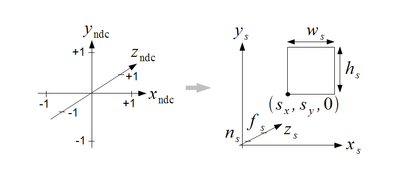
\includegraphics[scale = 1.2]{viewPort.png}
				\caption{视口变换图例}
				\label{shikou}
			\end{figure}
			
			在openGL视口变化通过函数: 
			\begin{lstlisting}
	glViewport(GLint sx , GLint sy , GLsizei ws , GLsizei hs); 
	glDepthRangef(GLclampf ns , GLclampf fs );
			\end{lstlisting}
			
			两个函数来指定。其中(sx,sy)表示\textbf{窗口的左下角},ns和 fs指定\textbf{远近剪裁平面到屏幕坐标的映射关系}。视口变换由OpenGL自动执行,不需要额外代码。
			
			
			
			
\chapter{光照}
	\section{颜色}
	
	\section{基础光照}
	
	\section{材质}
	
	\section{光照贴图}		
			
	\section{投光物}
	
	\section{多光源}
	
	\section{Gamma 矫正}
	
	\section{阴影}
	
	\section{法线贴图}
	
	\section{HDR}
	
	\section{延迟着色法}
	



\chapter{高级-特性}
	\section{模版测试}
	
	
	\section{深度测试}
	
	
	\section{混合}
	
	
	\section{面剔除}
	
	
	\section{帧缓冲}


	\section{立方体贴图}
	
	
	\section{几何着色器}
			
			
\chapter{OpenGL基础编程-API解释}
	
	\subsection{基本结构-框架}
		跟DirectX类似,都是进入消息循环然后不断监听消息。区别在于函数名可能不同,与其内部实现不同。
		有几个概念也是特别重要,其实这些就是数据准备过程和绘画过程,即Preparing to Send Data to OpenGL 和 Sending Data to OpenGL
		
		\begin{itemize}
			\item  顶点缓存对象(\textbf{Vertex Buffer Object,简称 VBO}[存在于内存中])
			\item  顶点缓存和索引缓存
			\item  缓存对象
			\item  reder()即display()
			\item 顶点数组对象 VAO (vertex array object)[显卡编程]
		\end{itemize}
		
		\subsubsection{创建顶点缓存}
			\begin{enumerate}
				\item 创建缓存对象,使用 glGenBuffers()
				\item 绑定缓存对象(指定使用哪一个缓存对象),使用 glBindBuffer()
				\item 拷贝顶点数据到缓存对象中,使用 glBufferData()
			\end{enumerate}
			
			\subparagraph{- void glGenBuffers(GLsizei n, GLuint* ids)}创建缓存对象,并返回缓存对象的标识符
				\begin{itemize}
					\item n :创建缓存对象的数量
					\item ids: 是一个 GLuint 型的变量或数组,用于储存缓存对象的单个 ID 或多个 ID
				\end{itemize}
				
			\subparagraph{- void glBindBuffer(GLenum target, GLuint id)}创建了缓存对象后,我们需要绑定缓存对象,以便使用。绑定,也就是指定当前要使用哪一个缓存对象,类似与DirectX的setStreamSource.
				\begin{itemize}
					\item target :缓存对象要存储的数据类型,只有两个值: GL\_ARRAY\_BUFFER, 和 GL\_ELEMENT\_ARRAY\_BUFFER。如果是顶点的相关属性,例如: 顶点坐标、纹理坐标、法线向量、颜色数组等,要使用 GL\_ARRAY\_BUFFER;索引数组,要使用 GL\_ELEMENT\_ARRAY\_BUFFER,以便 glDrawElements() 使用。
					
					\item id: 缓存对象的 ID
				\end{itemize}
			
			\subparagraph{- void glBufferData(GLenum target, GLsizei size, const void* data, GLenum usage)}拷贝数据到缓存对象,类似与DirectX的Lock操作.
				\begin{itemize}
					\item target: 缓存对象的类型,只有两个值: GL\_ARRAY\_BUFFER 和 GL\_ELEMENT\_ARRAY\_BUFFER
					
					\item size: 数组 data 的大小,单位是字节(bytes)
					\item data: 数组 data 的指针,如果指定为 NULL,则 VBO 只创建一个相应大小的缓存对象
					\item usage: 缓存对象如何被使用,有三中: 静态的(static)、动态的(dynamic)和流(stream).共有 9 个值:
						\begin{enumerate}
							\item GL\_STATIC\_DRAW
							\item GL\_STATIC\_READ
							\item GL\_STATIC\_COPY
							\item GL\_DYNAMIC\_DRAW
							\item GL\_DYNAMIC\_READ
							\item GL\_DYNAMIC\_COPY
							\item GL\_STREAM\_DRAW
							\item GL\_STREAM\_READ
							\item GL\_STREAM\_COPY
						\end{enumerate}
						
						\begin{itemize}
							\item Static: 指在缓存对象中的数据不能够更改(设定一次,使用很多次)
							\item Dynamic: 指数据将会频繁地更改(反复设定和使用)
							\item Stream: 指的是每一帧数据都会更改(设定一次,使用一次)
						\end{itemize}
						
						\begin{itemize}
							\item Draw: 指数据将会被送到 GPU 被用于绘制(application to GL)
							\item Read: 指数据将被读取到客户端应用程序(GL to application)
							\item Copy: 指数据将被用于绘制和读取(GL to GL)
						\end{itemize}
					\item 注意: Draw 只对 VBO 有用; Copy 和 Read 只对 PBO(像素缓存对象) 和 FBO(帧缓存对象) 有意义
				\end{itemize}
			
			\subparagraph{- void glBufferSubData(GLenum target, GLint offset, GLsizei size, void* data)}与 glBufferData() 一样,都是用于拷贝数据到缓存对象的。它能拷贝一段数据到一个已经存在的缓存,偏移量为 offset
			
			\subparagraph{- void glDeleteBuffers(GLsizei n, const GLuint* ids)}删除一个或多个缓存对象。
		
		
		\subsubsection{顶点缓存和索引缓存的使用}
			\subparagraph{1.准备顶点数据与索引数据}概念如同DirectX的绘制
				\begin{lstlisting}
	//顶点数据
	GLfloat vertexs[] = { 0.0f, 0.0f, 0.0f, 0.2f, 0.0f, 0.0f,
	-0.2f, 0.0f, 0.0f, 0.0f, 0.2f, 0.0f,
	0.0f, -0.2f, 0.0f, 0.0f, 0.0f, 0.2f,
	0.0f, 0.0f, -0.2f};
	
	//索引数据
	GLubyte indexs[] = {0,1,2,3,4,5,6};				
				\end{lstlisting}
			
			\subparagraph{2.生成缓存[数据,索引]对象,并拷贝数据}示例
				\begin{lstlisting}
	GLuint vboVertexId;
	GLuint vboIndexId;
	
	//生成数据缓存对象
	glGenBuffers(1, &vboVertexId);
	glBindBuffer(GL_ARRAY_BUFFER, vboVertexId);
	glBufferData(GL_ARRAY_BUFFER, sizeof(vertexs), vertexs, GL_STATIC_DRAW);
	
	//生成索引缓存对象
	glGenBuffers(1, &vboIndexId);
	glBindBuffer(GL_ELEMENT_ARRAY_BUFFER, vboIndexId);
	glBufferData(GL_ELEMENT_ARRAY_BUFFER, sizeof(indexs), indexs, GL_STATIC_DRAW);				
				\end{lstlisting}
				
			\subparagraph{3.使用}示例
				\begin{lstlisting}
	glEnableClientState(GL_VERTEX_ARRAY);
	glEnableClientState(GL_INDEX_ARRAY);
	
	glBindBuffer(GL_ARRAY_BUFFER, vboVertexId);
	glVertexPointer(3, GL_FLOAT, 0, 0);
	
	glBindBuffer(GL_ELEMENT_ARRAY_BUFFER, vboIndexId);
	glIndexPointer(GL_UNSIGNED_BYTE, 0, 0);
	
	//... 绘制图形
	
	glDisableClientState(GL_VERTEX_ARRAY); 
	glDisableClientState(GL_INDEX_ARRAY);
	glBindBuffer(GL_ARRAY_BUFFER, 0);				
				\end{lstlisting}
				
			\subparagraph{4.利用顶点绘图方法}示例
				\begin{lstlisting}
	//1. 第一种
	glBegin(GL_POINTS);
		glArrayElement(0);
		glArrayElement(1);
		glArrayElement(2);
		glArrayElement(5);
	glEnd();
	
	//2. 第二种  类似于DirectX的DrawPrimitive()函数
	glDrawElements(GL_POINTS, 7, GL_UNSIGNED_BYTE, 0);
	
	//3. 第三种
	glDrawArrays(GL_POINTS,0,7);				
				\end{lstlisting}
			
			\subparagraph{5.将不同类型的数据拷贝到一个缓存对象}缓存的一种用法,用 glBufferSubData() 可以将几个数据拷贝到一个缓存对象中
				\begin{lstlisting}
	GLfloat vertexs[] = {0.0f, 0.0f, 0.0f, 0.2f, 0.0f, 0.0f,
						-0.2f, 0.0f, 0.0f, 0.0f, 0.2f, 0.0f,
						0.0f, -0.2f, 0.0f, 0.0f, 0.0f, 0.2f,
						0.0f, 0.0f, -0.2f};
	
	GLfloat colors[] = {1.0f, 0.0f, 0.0f, 0.0f, 1.0f, 0.0f,
						0.0f, 0.0f, 1.0f, 1.0f, 1.0f, 0.0f,
						0.0f, 1.0f, 1.0f, 1.0f, 0.0f, 1.0f,
						0.0f, 0.0f, 0.0f};
	
	
	//现在,要将两个数组存在同一个缓存对象中,顶点数组在前,颜色数组在后
	glGenBuffers(1, &vboVertexId);
	glBindBuffer(GL_ARRAY_BUFFER, vboVertexId);
	glBufferData(GL_ARRAY_BUFFER, sizeof(vertexs)+sizeof(colors), 0, GL_STATIC_DRAW);
	glBufferSubData(GL_ARRAY_BUFFER, 0, sizeof(vertexs) , vertexs);    //注意第三个参数,偏移量
	glBufferSubData(GL_ARRAY_BUFFER, sizeof(vertexs), sizeof(colors), colors);
	
	
	//创建好缓存对象后,要用 glVertexPointer 和 glColorPointer 指定相应的指针位置。
	//但是,由于 glColorPointer 的最后一个参数,必须是指针类型。
	
	//glColorPointer 的最后一个参数用偏移量指示了颜色数组的位置
	glEnableClientState(GL_VERTEX_ARRAY);
	glEnableClientState(GL_COLOR_ARRAY);
	glEnableClientState(GL_INDEX_ARRAY);
	
	glBindBuffer(GL_ARRAY_BUFFER, vboVertexId);
	glVertexPointer(3, GL_FLOAT, 0, 0);
	glColorPointer(3,GL_FLOAT,0,(void*)sizeof(vertexs));    //注意最后一个参数
	
	glBindBuffer(GL_ELEMENT_ARRAY_BUFFER, vboIndexId);
	glIndexPointer(GL_UNSIGNED_BYTE, 0, 0);
	
	glDrawArrays(GL_POINTS,0,7);
	
	glDisableClientState(GL_VERTEX_ARRAY); 
	glDisableClientState(GL_COLOR_ARRAY); 
	glDisableClientState(GL_INDEX_ARRAY);
	glBindBuffer(GL_ARRAY_BUFFER, 0);				
				\end{lstlisting}
			
			\subparagraph{6.缓存对象的实时修改}在DirectX这个东西没搞出来,这竟然有个方法。
				比起显示列表,VBO 一个很大的优点是能够读取和修改缓存对象的数据。最简单的方法是重新拷贝虽有数据到 VBO,利用 glBufferData() 和 glBufferSubData(),这种情况下,你的程序必须要保存有两份数据:一份在客户端(CPU),一份在设备端(GPU)
				
				另一种方法,是\textbf{将缓存对象映射到客户端,再通过指针修改数据}
				
				 \textbf{- void* glMapBuffer(GLenum target, GLenum access)}
				 
					 映射当前绑定的缓存对象到客户端,glMapBuffer 返回一个指针,指向缓存对象。如果 OpenGL 不支持,则返回 NULL
				
					如果 OpenGL 正在操作缓存对象,此函数不会成功,直到 OpenGL 处理完毕为止。为了避免等待,可以先用 glBindBuffer(GL\_ARRAY\_BUFFER, 0) 停止缓存对象的应用,再调用 glMapBuffer
					
					\begin{itemize}
						\item target:GL\_ARRAY\_BUFFER 或 GL\_ELEMENT\_ARRAY\_BUFFER
						\item access:值有三个 GL\_READ\_ONLY、 GL\_WRITE\_ONLY、 GL\_READ\_WRITE,分别表示只读、只写、可读可写
					\end{itemize}
					
				\textbf{- GLboolean glUnmapBuffer(GLenum target)}
				
					修改完数据后,将数据反映射到设备端
					
				\begin{lstlisting}
	glBindBuffer(GL_ARRAY_BUFFER, vboVertexId);
	GLfloat* ptr = (float*)glMapBuffer(GL_ARRAY_BUFFER, GL_WRITE_ONLY);
	
	if(ptr)
	{
		ptr[0] = 0.2f;  ptr[1] = 0.2f;  ptr[2] = 0.2f;
		glUnmapBuffer(GL_ARRAY_BUFFER);
	}
	
	glBindBuffer(GL_ARRAY_BUFFER, 0);				
				\end{lstlisting}
		\subsubsection{顶点缓存和顶点数组的使用:VAO、VBO}
			\subparagraph{VAO}是这样一种方式:\textbf{把对象信息直接存储在图形卡中},\textit{而不是在当我们需要的时候传输到图形卡}。这就是Direct3D所采用得方式,而在OpenGL中只有OpenGL3.X以上的版本中采用。这就意味着我们的应用程序不用将数据传输到图形卡或者是从图形卡输出,这样也就获得了额外的性能提升.
			
			\subparagraph{使用}使用VAO并不难。我们不需要大量的glVertex调用,而是把顶点数据存储在数组中,然后放进VBO,最后在VAO中存储相关的状态。记住:VAO中并没有存储顶点的相关属性数据。OpenGL会在后台为我们完成其他的功能。
				\begin{enumerate}[itemindent = 1em]
					\item \textbf{产生VAO}:\textit{void glGenVertexArrays(GLsizei n,GLuint *arrays);}
						\begin{itemize}
							\item n:要产生的VAO对象的数量
							\item arrays:存放产生的VAO对象的名称
						\end{itemize}
						
					\item \textbf{绑定VAO}: \textit{void glBindVertexArray(GLuint array)};
						\begin{itemize}
							\item arrays:要绑定的顶点数组的名字
						\end{itemize}
						
					\item \textbf{产生VBOs}: \textit{void glGenBuffers(GLsizei   n,GLuint *   buffers)};参考上
					\item \textbf{绑定VBOs}:\textit{void glBindBuffer(GLenum   target,GLuint   buffer)};
					
					\item \textbf{给VBO分配数据}:\textit{void glBufferData( GLenum target,GLsizeiptr size,const GLvoid *  data,GLenum   usage)};
						\begin{itemize}
							\item target可能取值为:
								\begin{itemize}
									\item GL\_ARRAY\_BUFFER(表示顶点数据)
									\item GL\_ELEMENT\_ARRAY\_BUFFER(表示索引数据)	
									\item GL\_PIXEL\_PACK\_BUFFER(表示从OpenGL获取的的像素数据)
									\item GL\_PIXEL\_UNPACK\_BUFFER(表示传递给OpenGL的像素数据)
								\end{itemize}
							\item size:缓冲区对象字节数
							\item data:指针:指向用于拷贝到缓冲区对象的数据。或者是NULL,表示暂时不分配数据
						\end{itemize}
					\item \textbf{定义存放顶点属性数据的数组,启用VAO中对应的顶点属性数组},\textit{void glEnableVertexAttribArray( GLuint  index)}
					
					\item \textbf{给对应的顶点属性数组指定数据}:\textit{void glVertexAttribPointer(GLuint  index,GLint size,GLenum  type,GLboolean  normalized,GLsizei  stride,const GLvoid*  pointer)};
					
					\item \textbf{然后在进行渲染的时候,只需要绑定对应的VAO即可}:\textit{glBindVertexArray(vaoHandle)};
					
					\item \textbf{使用完毕之后需要清除绑定}:\textit{glBindVertexArray(0)};
				\end{enumerate}
		\subsubsection{使用VAO Mesh 类示例}
			\subparagraph{VAO[直接使用图形卡缓存绘图]-代码}示例如下:
			\begin{lstlisting}
	// 顶点
	class Vertex{
	public:
		Vertex(const glm::vec3& pos):this->pos = pos{}
	private:
		glm::vec3 pos;
	};
	
	// 网格
	class Mesh{
	public:
		Mesh(Vertex* vertices, unsigned int numVertices)
		{
			m_drawCount = numVertices;
			
			glGenVertexArrays(1, &m_vertexArrayObject);
			glBindVertexArray(m_vertexArrayObject);
			
			glGenBuffers(NUM_BUFFERS, m_vertexArrayBuffers);
			glBindBuffer(GL_ARRAY_BUFFER, m_vertexArrayBuffer[POSITION_VB]);
			glBufferData(GL_ARRAY_BUFFER, numVertices * sizeof(vertices[0]), vertices, GL_STATIC_DRAW);
			
			glEnableVertexAttribArray(0);
			glVertexAttribPointer(0,3, GL_FLOAT, GL_FALSE, 0, 0);
			
			glBindVertexArray(0);
		}
		~Mesh()
		{
			glDeleteVertexArrays(1, &m_vertexArrayObject);
		}
		
		void Draw()
		{
			glBindVertexArray(m_vertexArrayObject);
			
			glDrawArrays(GL_TRIANGLES, 0, m_drawCount);// 第三个参数为总共的 顶点个数,当然画三角形s,就是3的倍数咯
			
			glBindVertexArray(0);
		}
	private:
		enum{
			POSTION_VB,
			NUM_BUFFERS
		};
		GLuint m_vertexArrayObject;
		GLuint m_vertexArrayBuffer[NUM_BUFFERS];
		usigned int m_drawCount;
	};
	
	// Main 调用Mesh Draw
		Vertex vertices[] = {Vertex(glm::vec3(-0.5,-0.5,0)),
							 Vertex(glm::vec3(0,0.5,0)),
							 Vertex(glm::vec3(0.5,-0.5,0)),}
							 
		Mesh mesh(vertices, sizeof(vertices)/sizeof(vertices[0]));
			\end{lstlisting}
			
		\subparagraph{结果}
			实现结果见图\ref{VAOResult}:
			\begin{figure}[h]
				\centering
				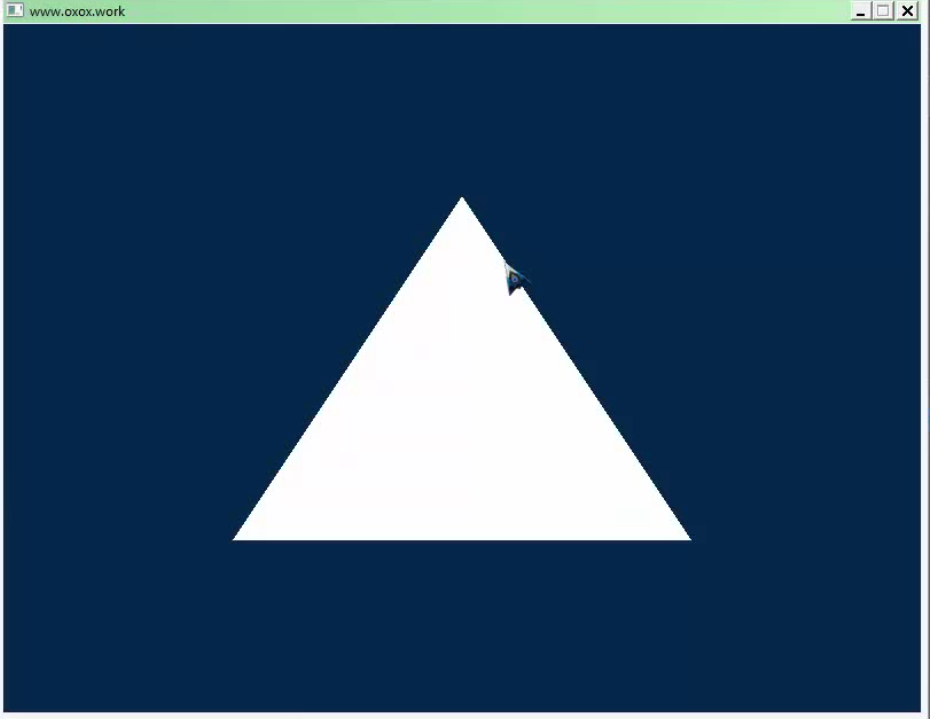
\includegraphics[scale = 0.5]{VBOMeshResult.png}
				\caption{上述Mesh代码绘画效果}
				\label{VAOResult}
			\end{figure}
	
	
	
	\section{API-VAO、VBO、EBO}
		\subsection{glVertexAttribPointer()}
			\begin{lstlisting}
void glVertexAttribPointer(	
	GLuint index,
 	GLint size,
 	GLenum type,
 	GLboolean normalized,
 	GLsizei stride,
 	const GLvoid * pointer);			
			\end{lstlisting}

			
		

\chapter{MFC with OpenGL}
	\section{环境配置}
		\url{http://blog.csdn.net/sircarfield/article/details/6992586}
		
		\url{http://www.cnblogs.com/phinecos/archive/2007/07/28/834916.html}
		
	\section{闪烁解决办法}
		\url{http://blog.sina.com.cn/s/blog_6d4b374e010141ix.html}
		    
		\url{http://bbs.csdn.net/topics/390804673}
			
	\section{定时器概念与程序}
		\url{http://blog.sina.com.cn/s/blog_678e97f80100thp7.html}
			
			
	\section{坐标确定}
		左下角为原点
		
	\section{画椭球}
		\url{http://www.tuicool.com/articles/zmE3Mr}
		

\chapter{OpenGL 读取 OBJ 文件}
    \section{参考文献} 
		\subparagraph{OBJ 文件格式}\url{http://guanser.blog.163.com/blog/static/2112467872012877161702/}
	
	
 
\chapter{OpenGL 实现天空盒子}
	\section{实现}
		
	\section{错误记录}
		\paragraph{1.error LNK1281}error LNK1281: 无法生成 SAFESEH 映像VS2013常见编译错误解决
		
		\subparagraph{解决方案}:
		
		打开项目属性的链接器的命令行,在那里输入: /SAFESEH:NO点击确定再次编译,成功解决问题


\chapter{PCL  安装}
	\section{错误记录}
		\paragraph{1.error LNK2019} 要么是 依赖库没配置好, 要么就是32位与64位不兼容(这里包括 库与系统不兼容,还包括库与系统兼容但与编译器不兼容)
		
		如当使用 64位的库时,也是64位的系统,虽然你使用的编译器也是64位,但是在编译的时候并没有选择 x64,而选择了win32 也会出现这个错误
		
		参考该文章的更改编译器部分\url{http://www.ithao123.cn/content-8701571.html}
\end{document} 
 		    